\chapter{Effects of localised shearing on crystal growth and nucleation}
As outlined in Chapter 1, the original outline of the project is to 
investigate the possibility of using optical tweezing to induce nucleation 
by generating fluid flow within a supersaturated solution. The intent 
of which would be twofold: Firstly to have a repeatable means of 
inducing nucleation under different solution conditions. And secondly, 
to understand the influence of shearing on nucleation at a micro 
level as compared to results in bulk fluid. It has been shown that 
for macro-scale systems, the likelihood of nucleation increases to 
a maximum value under increased shearing \cite{Debuysschere2023, 
Mura2016}. Mura and Zaccone developed a theoretical framework to 
describe how the a newly formed nucleus experiences two additional 
growth factors when placed in a moving fluid. Firstly, due to increased 
molecular transport of solute molecules the nucleation rate is enhanced 
in low to moderate fluid flows. But in addition, due to shear flow the 
crystal surface undergoes deformation which suppresses the nucleation 
rate undergoing faster fluid flow \cite{Mura2016}. The theory was 
confirmed for glycine solution by Debuysschere \textit{et al} who
identified that the nucleation rate of supersaturated glycine was 
enhanced up until $\dot{\gamma}\approx3000\ s^{-1}$ \cite{Debuysschere2023}.
After which the nucleation rate began to decrease but was 
still greater compared to the case where fluid flow was minimal.

Optical tweezers can been used to rotate a whole host of micro-rotors, 
with the fastest reported results exceeding $1000\ Hz$ in heavy water
\cite{Arita2016}. Therefore, it stands to reason that a micro-rotor
rotating in a supersaturated solution could generate sufficient fluid
flow such that the nucleation rate around said particle is enhanced 
compared to the bulk fluid. We focused on two primary candidates for
micro-rotors, Vaterite and 4-Heptyl-4-biphenylcarbonitrile (7CB). The
former being a polymorph of calcium carbonate and the latter an example
of nematic liquid crystals, both of which have been used repeatedly in
previous micro-rotor. In addition, we also consider the application of
using techniques beam steering to generate fluid flow by trapping silica
micro-beads. In this instance the fluid flow is generated not due to the
transfer of angular momentum, but due to shearing caused by a moving 
sphere through stagnant fluid.

To begin with, the discussion of the necessary optical equipment is 
covered, drawing attention to specialised components and techniques 
that are not standard in optical trapping set ups.
%%%%%%%%%%%%%%%%%%%%%%%%%%%%%%%%%%%%%%%%%%%%%%%%%%%%%%%%%%%%%%%%%%%%%%%%%%%%%%%%
%%%%%%%%%%%%%%%%%%%%%%%%%%%%%%%%%%%%%%%%%%%%%%%%%%%%%%%%%%%%%%%%%%%%%%%%%%%%%%%% 
\section{Optical Tweezer Equipment}
In general, all optical tweezers require a laser driver, a focusing 
microscope objectives, a position controller, and position detector.
The laser used for this project was a $1064\ nm$ near infrared laser 
- provided by CNI Lasers – that was focused by a Nikon 100x oil 
immersion lens. The choice of an oil immersion lens is important as 
the optical oil used prevents a loss of focus when used on a glass 
cover slip. Now, experimental work has shown that the trapping 
efficiency increases with beam diameter up until it exceeds 
$\frac{2}{3}D_{obj}$ \cite{kim2003dependence} where $D_{obj}$ is 
the diameter of the objective aperture. To expand the beam front we 
utilise a Galilean beam expansion arrangement (indicated by $f_1$, 
and $f_2$ in Fig.~\ref{fig:setup}) as recommended for high power laser 
applications. In our initial experiments the beam expansion provides a 
$4\times$ magnification. Whereas in later experiments we utilised a 
galvano-mirror the beam expansion is $3\times$ and then the 4f 
correlator provides a further $1.25\times$ magnification (using $f_3$ 
and $f_4$) - the magnification is given by.
\begin{align}
	\frac{D_2}{D_1} = \frac{f_2}{f_1}
\end{align}

It should be noted that the galvano-mirror requires the use of a 
Keplerian beam expansion arrangement which reduces the transmitted 
laser power due to localised heating of the air. Afterwards the 
laser is passed through a dichroic mirror that separates incoming 
infrared and visible light, this is to prevent the laser from 
damaging the CCD camera used for imaging the trapping plane. The 
laser is then focused to a diffraction limited spot by the objective. 
Utilizing a high numerical aperture objective enhances the gradient 
force at the focal point; the trade-off being that the for higher NA 
objectives the trapping depth is reduced due to spherical aberrations. 
While it is possible to increase the trapping depth \cite{Reihani2006} 
by adjusting the objective's tube length this approach is incompatible 
with our trapping arrangement. A 0.25 NA condenser objective refocuses 
the scattered laser light and also provide an aperture for an imaging 
LED to illuminate the focal plane. Samples are loaded onto a piezo 
driven table to that is inserted between the trapping and condensing 
objectives; the piezo drivers allow for sub-micron control of the 
beam focus position to a degree as small as a 10 nm. To detect and 
monitor the position of a trapped particle a quadrant photo diode 
(QPD) was utilised. 
\begin{figure}[h!]
	\centering
	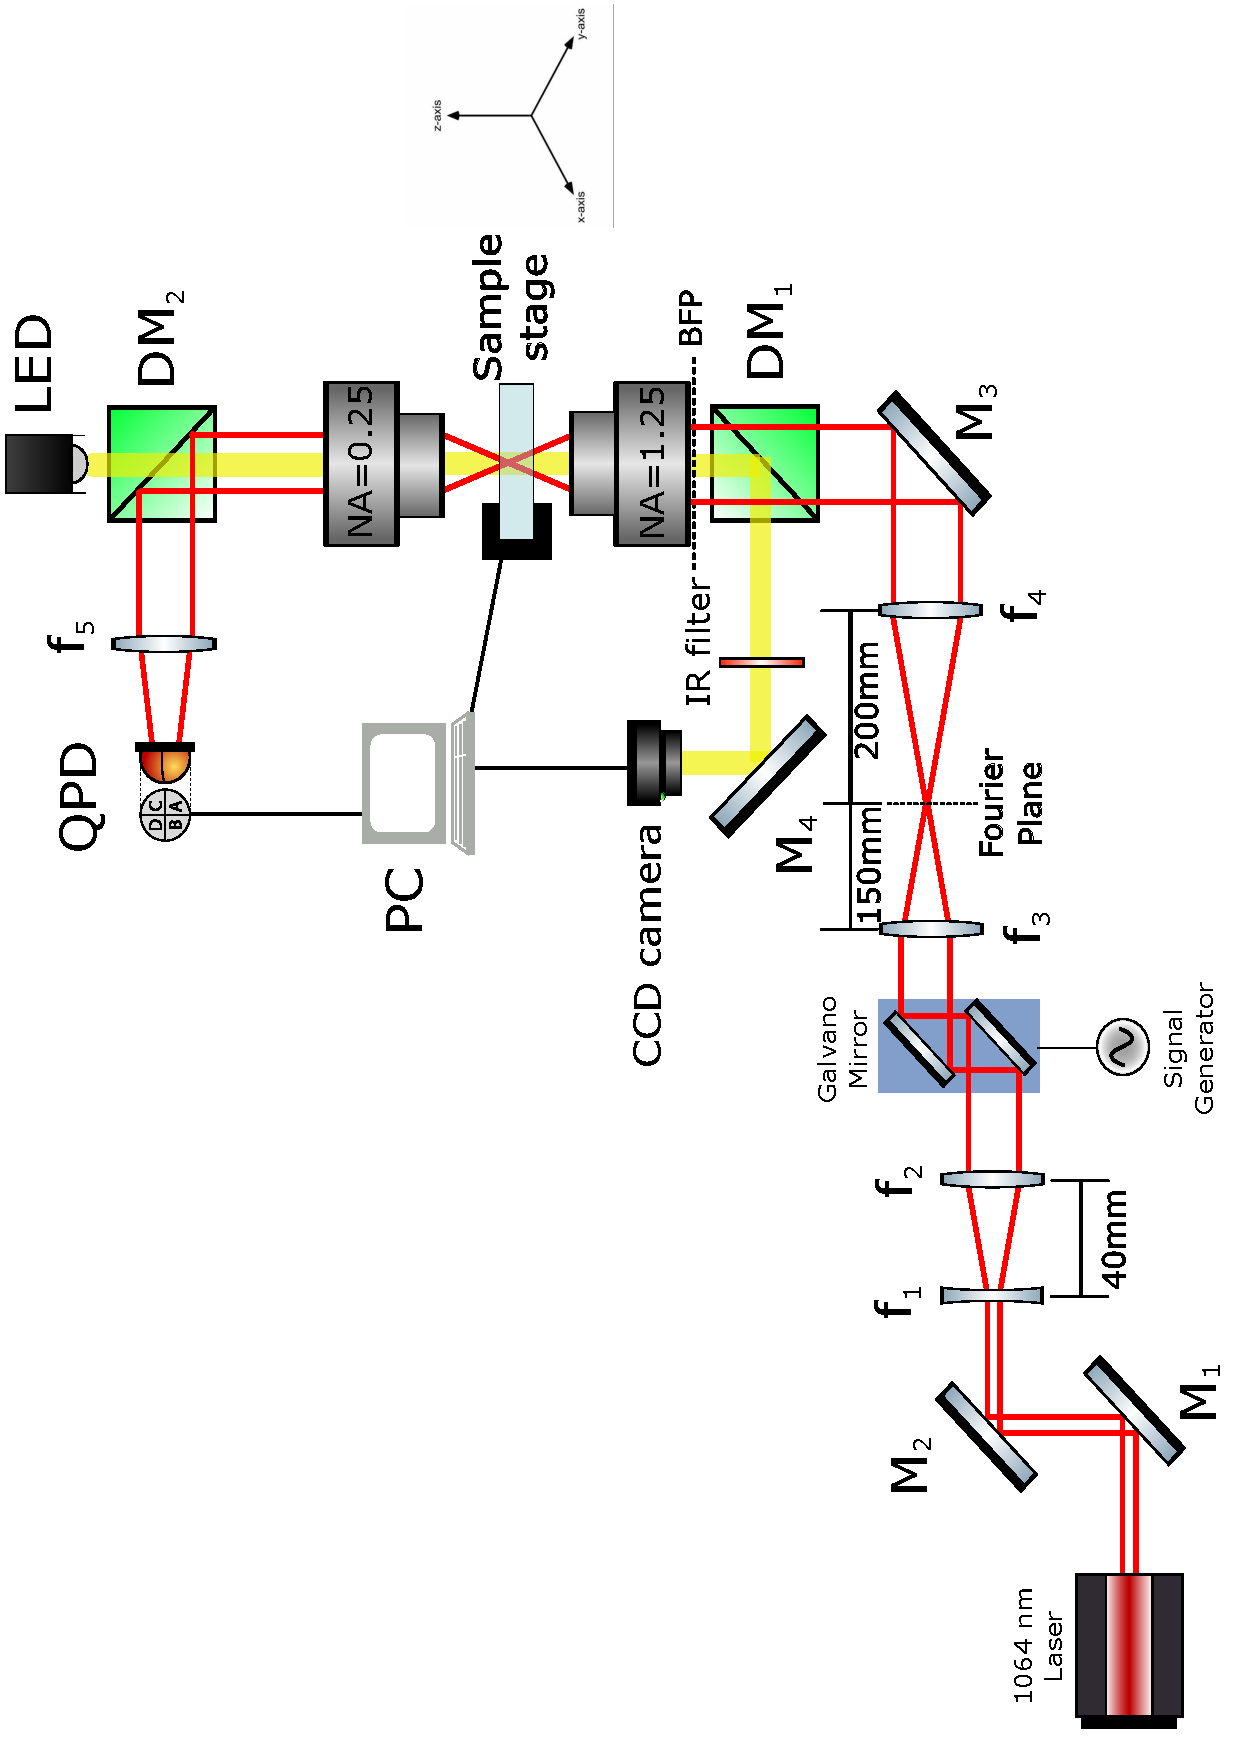
\includegraphics[height=\linewidth, angle=270]{tweezer_setup.pdf}
	\caption{Optical tweezer set up used for the majority of the PhD. The focal lengths of $f_1$, $f_2$, $f_3$, \& $f_4$ are $-20\ mm$, $60\ mm$, $150\ mm$, \& $200\ mm$ respectively. Diagram not drawn to scale.}
	\label{fig:setup}
\end{figure}

%%%%%%%%%%%%%%%%%%%%%%%%%%%%%%%%%%%%%%%%%%%%%%%%%%%%%%%%%%%%%%%%%%%%%%%%%%%%%%%%
\subsection{Position detection methods}
In order to accurately capture the dynamics of a trapped particle, a 
position detection system is required. There are 3 possible methods 
of position detection: video-analysis, lateral-effect position sensing, 
and photodiodes. The former being ideally suited for multiple traps 
or situations where precision is not the top priority. In order to 
match the force measurements of back-focal plane interferometry requires 
the camera's frame rate to exceed $1\ kHz$ which can be difficult 
to achieve while maintaining a decent resolution \cite{Gibson2008}. 
In comparison off the shelf back-focal plane detectors can achieve 
temporal resolutions anywhere from $10-100\ kHz$ \cite{BergSoerensen2004}. 
 
A quadrant photo diode (QPD) is a frequently used position detection 
system for optical tweezers due to their high sampling rate, high 
degree of precision, and ease of set up. The QPD is constructed of 
four photo diodes assembled in a quadrant formation, when a particle 
is trapped the interference pattern produced is focused onto the QPD, 
with the maximum intensity mapping to the particle's centre of mass. 
By summing the voltages of the horizontal and vertical quadrants together 
the particle's centre of mass is tracked in the x-y plane. Axial 
displacement can be estimated by observing the change in the total 
voltage of the QPD. The outputted signal gives an indication of the 
particle's relative displacement from the beam focus, but in order to 
convert the signal to distance units the trap needs to be calibrated 
(assuming a linear response curve).
\begin{figure}[h!]
	\centering
	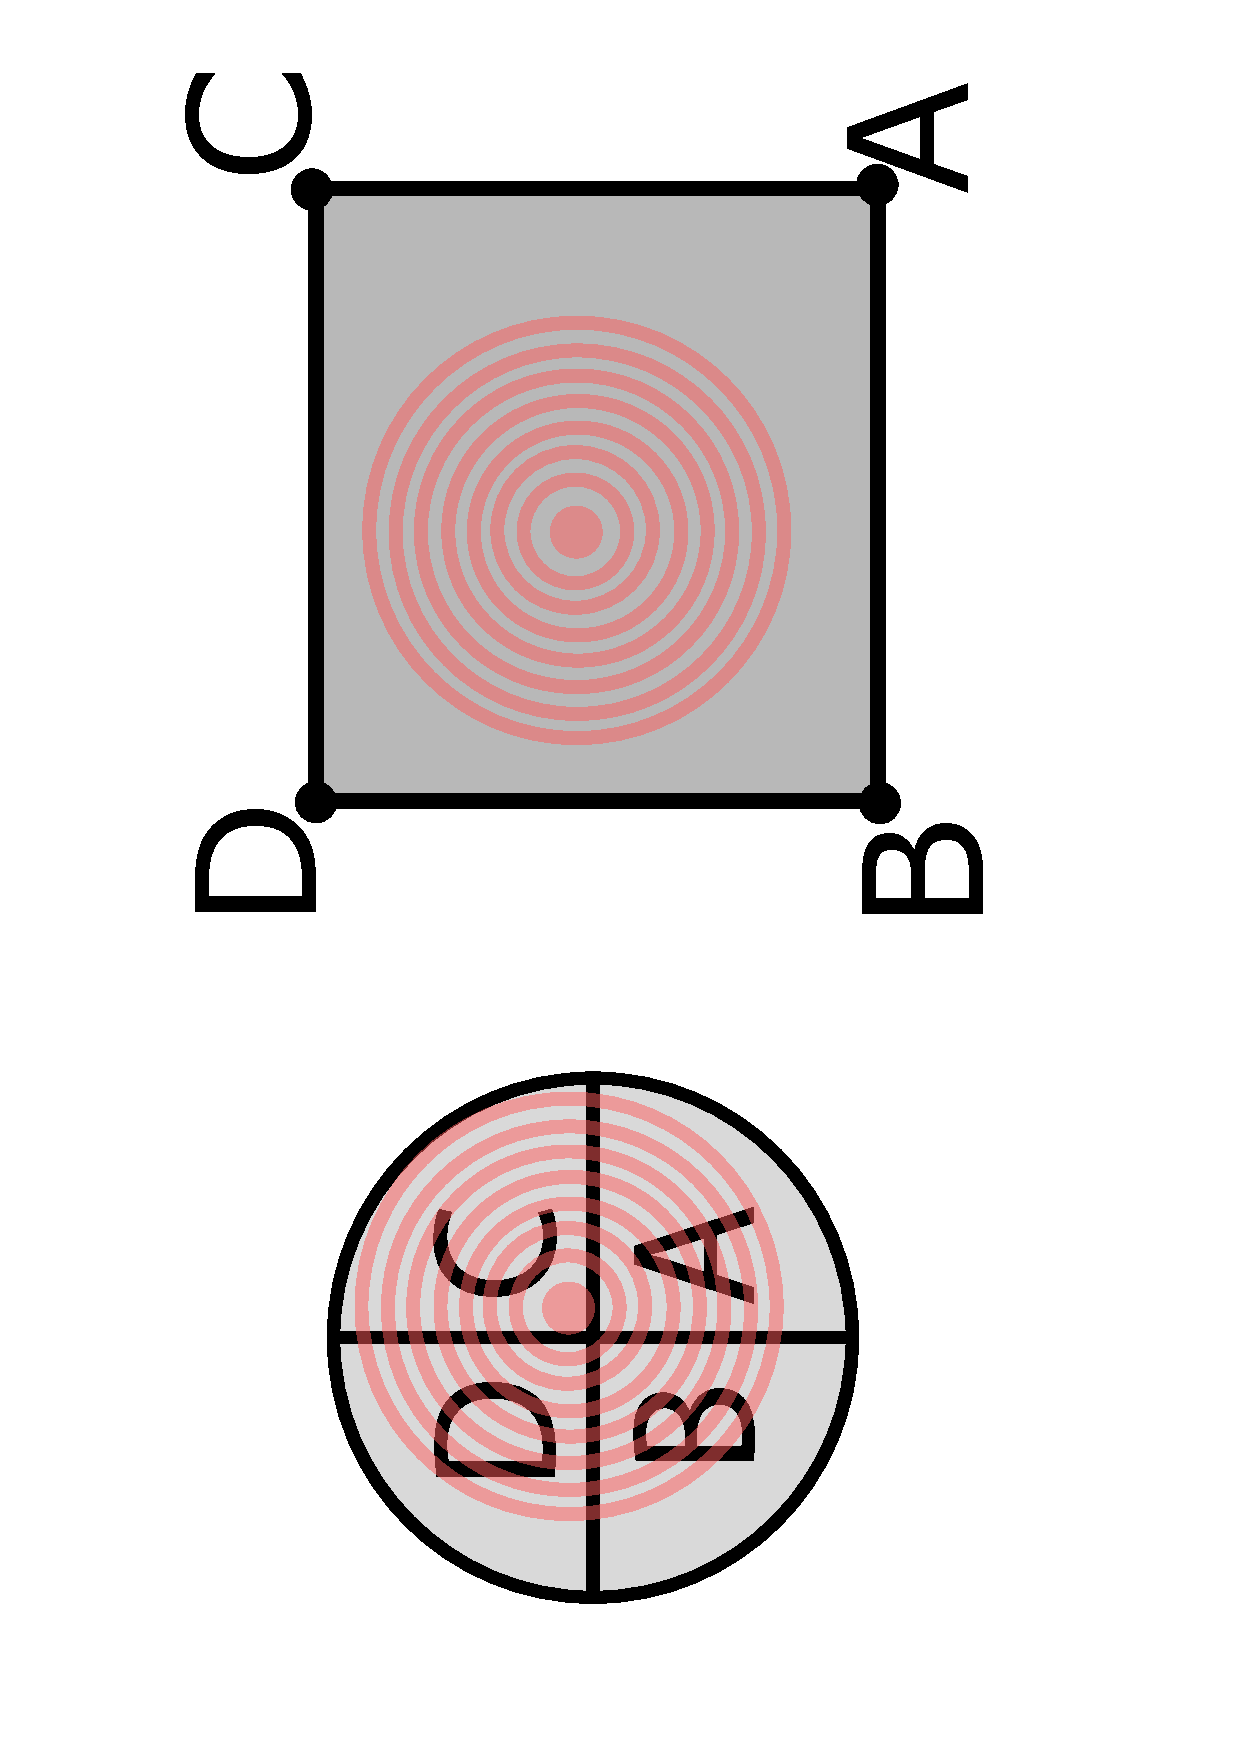
\includegraphics[height=\linewidth, angle=270]{QPD_Lateral_effect.pdf}
	\caption{Comparison between QPD and Lateral effect photodiodes.
	The four quadrants of a QPD (left) experience different photocurrents
	based on the total intensity of light incident on each section 
	(labelled A, B, C, D). 
	Whereas a Lateral effect sensor (right) uses the resistive properties
	of the photodiode surface to vary the create different photocurrents 
	passing through the anodes A, B, C, and D.}
\end{figure}

A lateral-effect sensor has a similar output but works using a the 
entire sensor as a single cell analogous to the focal plane of the 
trapping beam. The four corners of the sensor act as anodes connected 
to a base plate cathode, as the beam moves across the surface of the 
detector each anode will experience a different photocurrent depending 
on how close the centre of the interference pattern is to each anode. 
The advantage of a lateral effect detector is that the linear regime 
is much larger than a QPD making it much better for monitoring the 
position of a trapped particle. However, Lateral-effect sensors are 
often limited in their spacial resolution due to high signal-to-noise 
ratios, requiring a high intensity of light on the sensor in order to 
get a clean signal. As a result, most optical force measurements are 
conducted using a QPD as opposed to a lateral-effect sensor, as often 
the displacement is small enough that the signal-displacement curve 
can be considered linear.

%%%%%%%%%%%%%%%%%%%%%%%%%%%%%%%%%%%%%%%%%%%%%%%%%%%%%%%%%%%%%%%%%%%%%%%%%%%%%%%%
\subsection{Fourier Optics and 4f correlators}
A 4f correlator is an example of Fourier optics in practice, understanding
that a focused lens takes a Fourier transform of the light profile. 
Consider a laser with a circular Gaussian profile, if you were to place 
a detector there you would pick up the intensity as a function of its 
position within the beam. If however you focused the light into a single 
point (using a +ve focal lens) you are actually seeing a measurement of 
the phase of your laser with position, in which you would see a diffraction
limited spot ($d = \lambda/2nsin(\theta)$), indicating that the laser is 
collimated. In imaging systems, a series of focal lenses can be used to 
filter out unwanted scattering from an image (or in an inverse case 
differentiate between different images), the placement of each lens is 
shown below.
\begin{figure}[h!]
	\centering
	\begin{subfigure}{0.475\linewidth}
		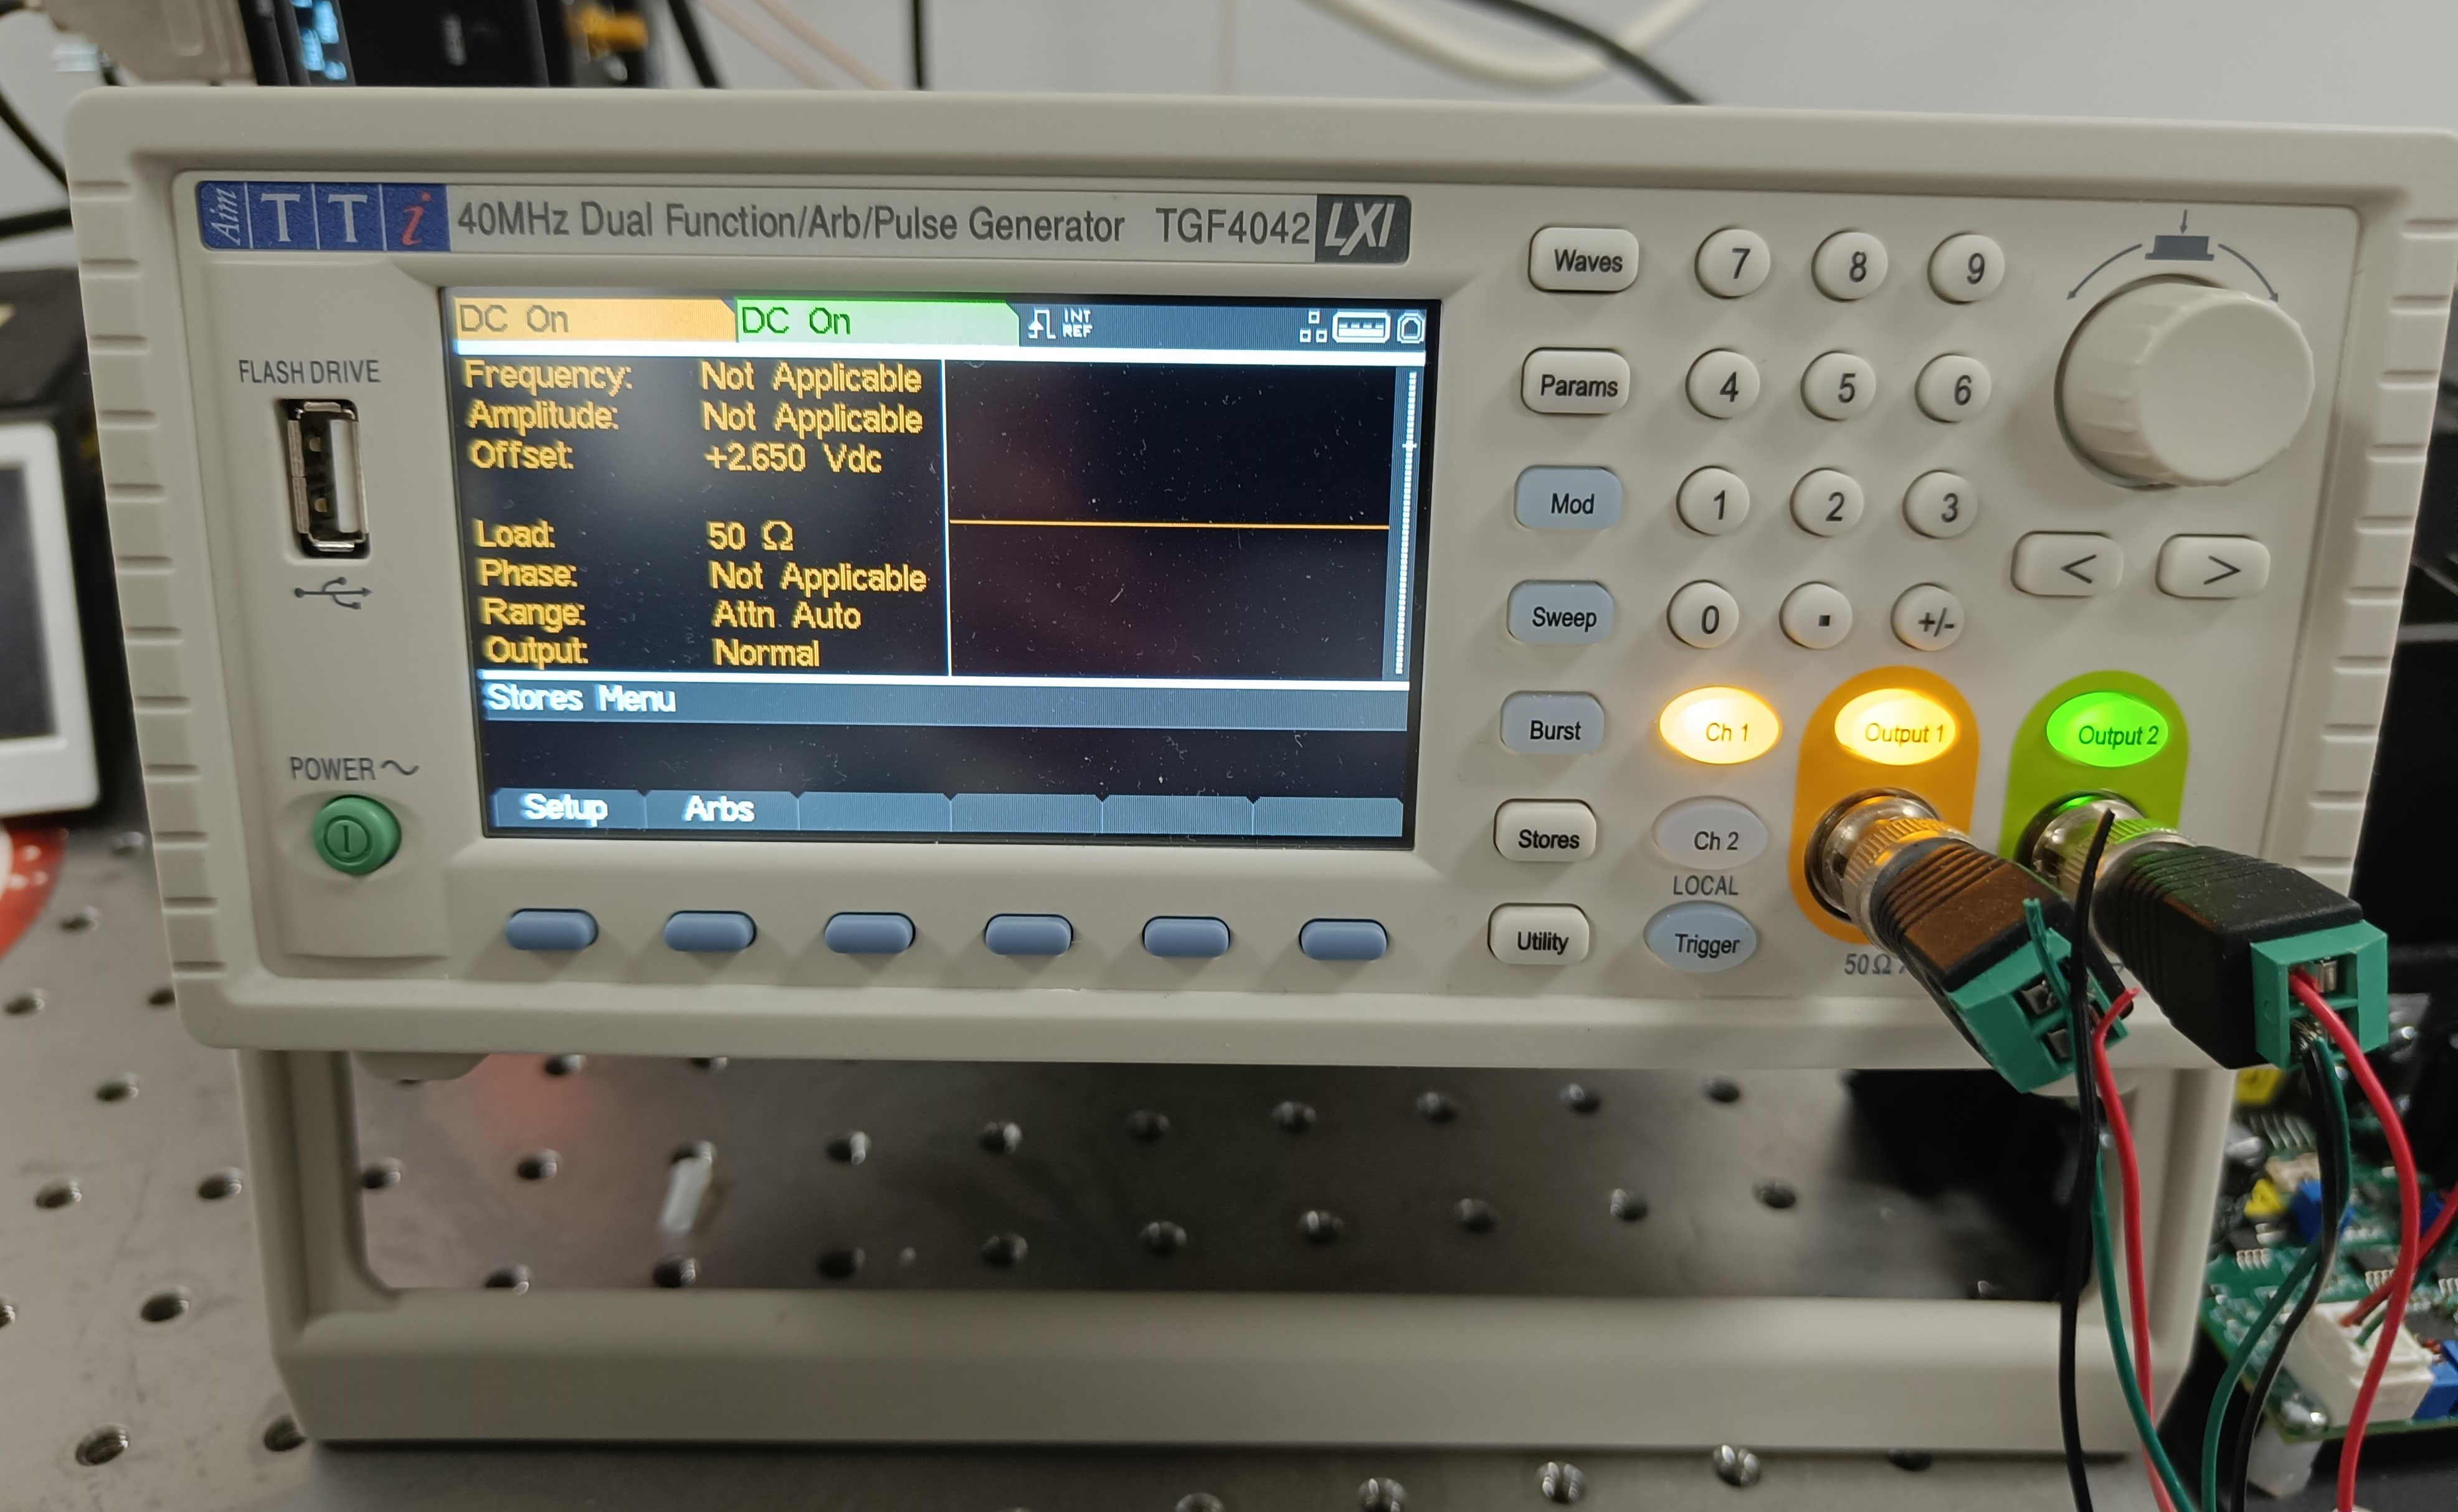
\includegraphics[width=\linewidth]{signal_generator.jpg}
		\caption{}
	\end{subfigure}
	\begin{subfigure}{0.475\linewidth}
		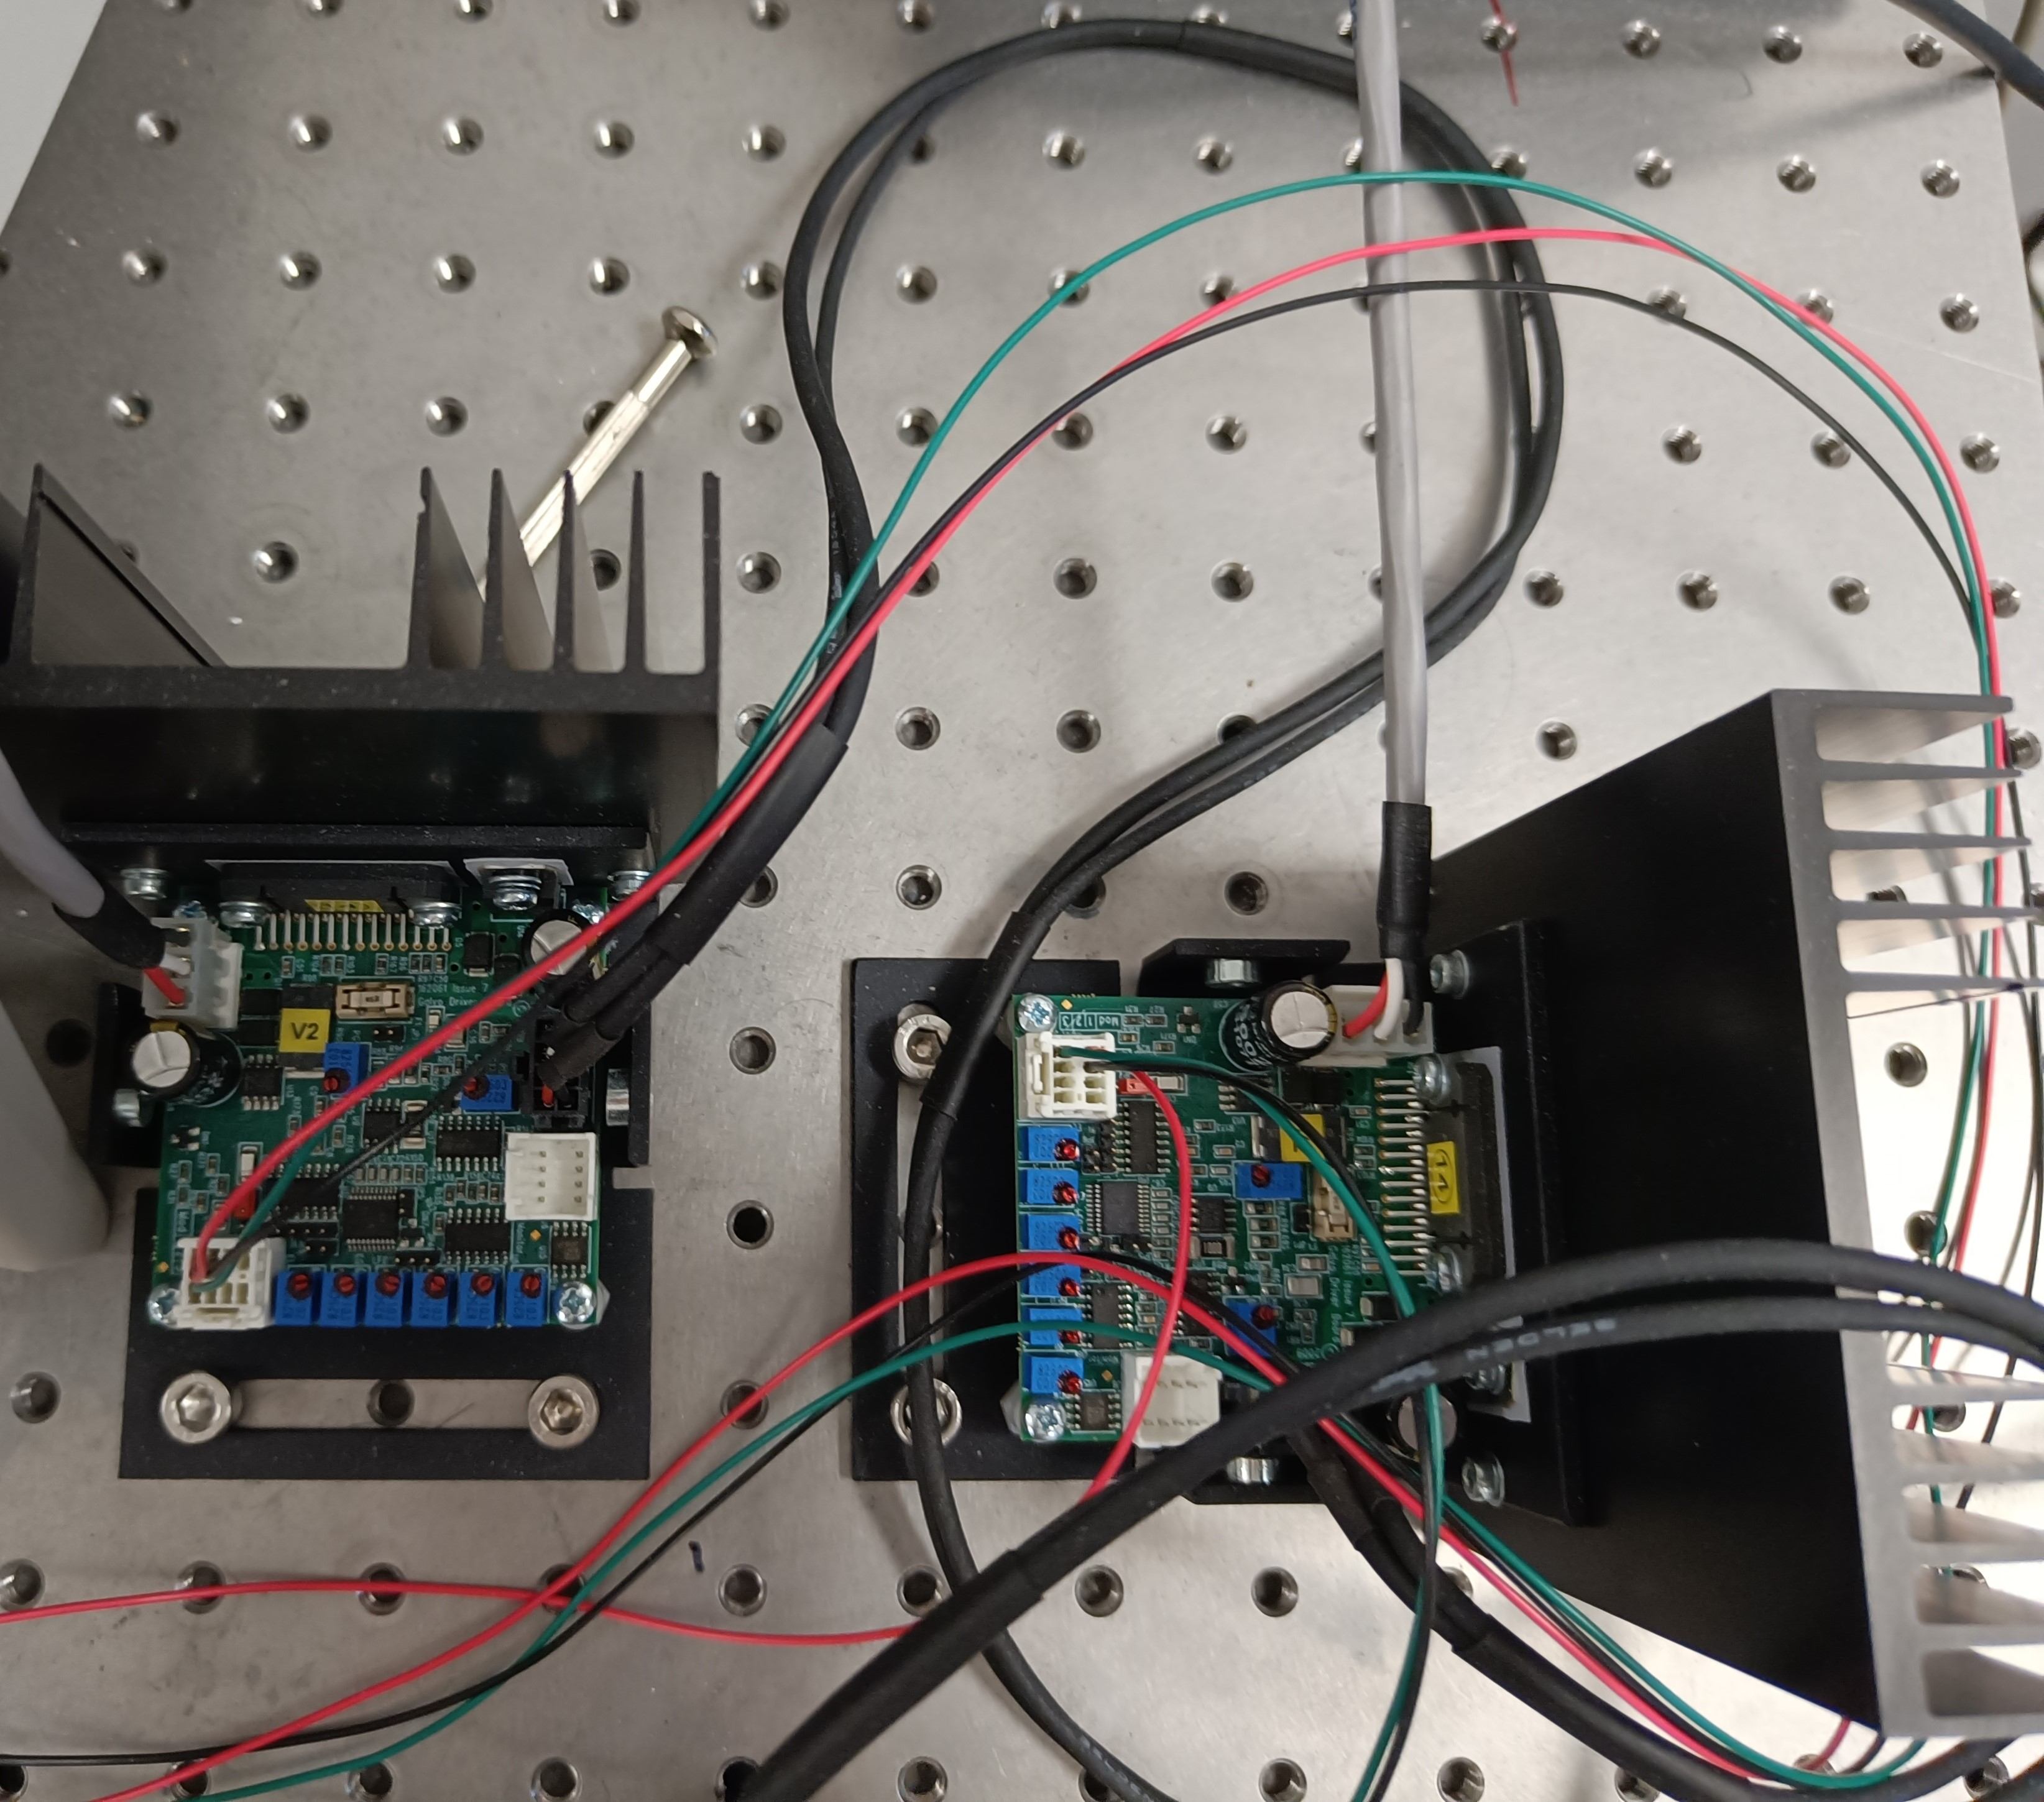
\includegraphics[width=\linewidth, height=0.7\linewidth]
		{galvano_mirror_controllers.jpg}
		\caption{}
	\end{subfigure}

	\caption{Signal generator galvano mirror controller, channel 1 controls the x-axis 
		mirror, while channel 2 controls the y-axis mirror. Both channels can be manipulated
		independently.}
\end{figure}

For our applications a 4f correlator is utilised to ensure that the motion
of the galvano-mirrors does not move the focal point of the laser, allowing 
for a stable trap even while in motion. As shown in Fig.~\ref{fig:setup}, after
the galvano-mirror we have our two lenses - $f_3$ and $f_4$ - the former being 
installed $150\ mm$ from the second mirror of the galvano, and the latter being 
installed $200\ mm$ from the back focal plane of the trapping objective. The 
signal generator used was supplied by 'MCS Test Equipment Ltd', allowing for 
dual channel signal control. This allowed us to precisely control the alignment,
amplitude, phase, and frequency of both mirrors making alignment much easier. For
basic trapping calibration the galvano-mirrors were set to a simple DC output, 
providing a fixed spot which operates like a typical optical trap.

%%%%%%%%%%%%%%%%%%%%%%%%%%%%%%%%%%%%%%%%%%%%%%%%%%%%%%%%%%%%%%%%%%%%%%%%%%%%%%%%
%%%%%%%%%%%%%%%%%%%%%%%%%%%%%%%%%%%%%%%%%%%%%%%%%%%%%%%%%%%%%%%%%%%%%%%%%%%%%%%%
\section{Synthesis of Birefringent Micro spheres}
\label{sec:vaterite}
There are several options for particles that can be rotated using optical 
tweezers \cite{Parkin2009, Saito2022}. Over the course of the project two 
different micro spheres where investigated, Vaterite and liquid crystal 
droplets. Both can be readily synthesised in the lab and are will rotate 
at a variety of sizes.

Vaterite is a polymorph of calcium carbonate that is rarely seen in nature 
due to its low stability \cite{KonopackaLyskawa2019}. However unlike its 
other polymorphs of calcite and aragonite, when synthesised Vaterite will 
typically form small spherical particles making them ideal for optical 
trapping and rotation. Synthesis of Vaterite micro spheres requires fine 
control of the crystal growth process in order to maintain polymorphic stability. 
Though for the purposes of optical rotation the exact polymorph is not as 
important as its morphology as all 3 polymorphs are inherently birefringent. 

Vaterite samples where made by the first preparing equal amounts of 
$CaCl_2$ and $Na_2CO_3$ at a concentration of $0.33M$, at the same time
a vial of $0.33M\ MgSO_4$ was prepared and set aside for later. First
a small vial was filled with $1.5mL$ of $CaCl_2$ followed by $60\mu L$ 
and $90\mu L$ of $MgSO_4$ and $NaCO_3$ respectively, forming a seed solution. 
Next, a larger vial was filled with $5\ mL$, $1.5\ mL$, and $1\ mL$ of
$CaCL_2$, $MgSO_4$, and $NaCO_3$ respectively followed by the seed solution. 
After 10 minutes of slow but continuous mixing a few drops of Agepon was added
to halt the reaction, the solution was filtered and washed 3 times with 
distilled water before being suspended in water.
 
When trapped in circularly polarised light, the anisotropic crystal lattice
allows spin angular momentum to be transferred to the Vaterite particle, 
resulting in a rotation about the beam axis. In addition, the anisotropic 
scattering causes the QPD signal to vary with a constant periodicity that
is attributed to its rotation rate. Therefore, the resulting power spectrum 
is not a Lorentzian but now also displays peaks that appear at integer 
multiples of the particles rotational frequency. 
\begin{figure}[h!]
	\centering
	\begin{subfigure}{0.4\linewidth}
		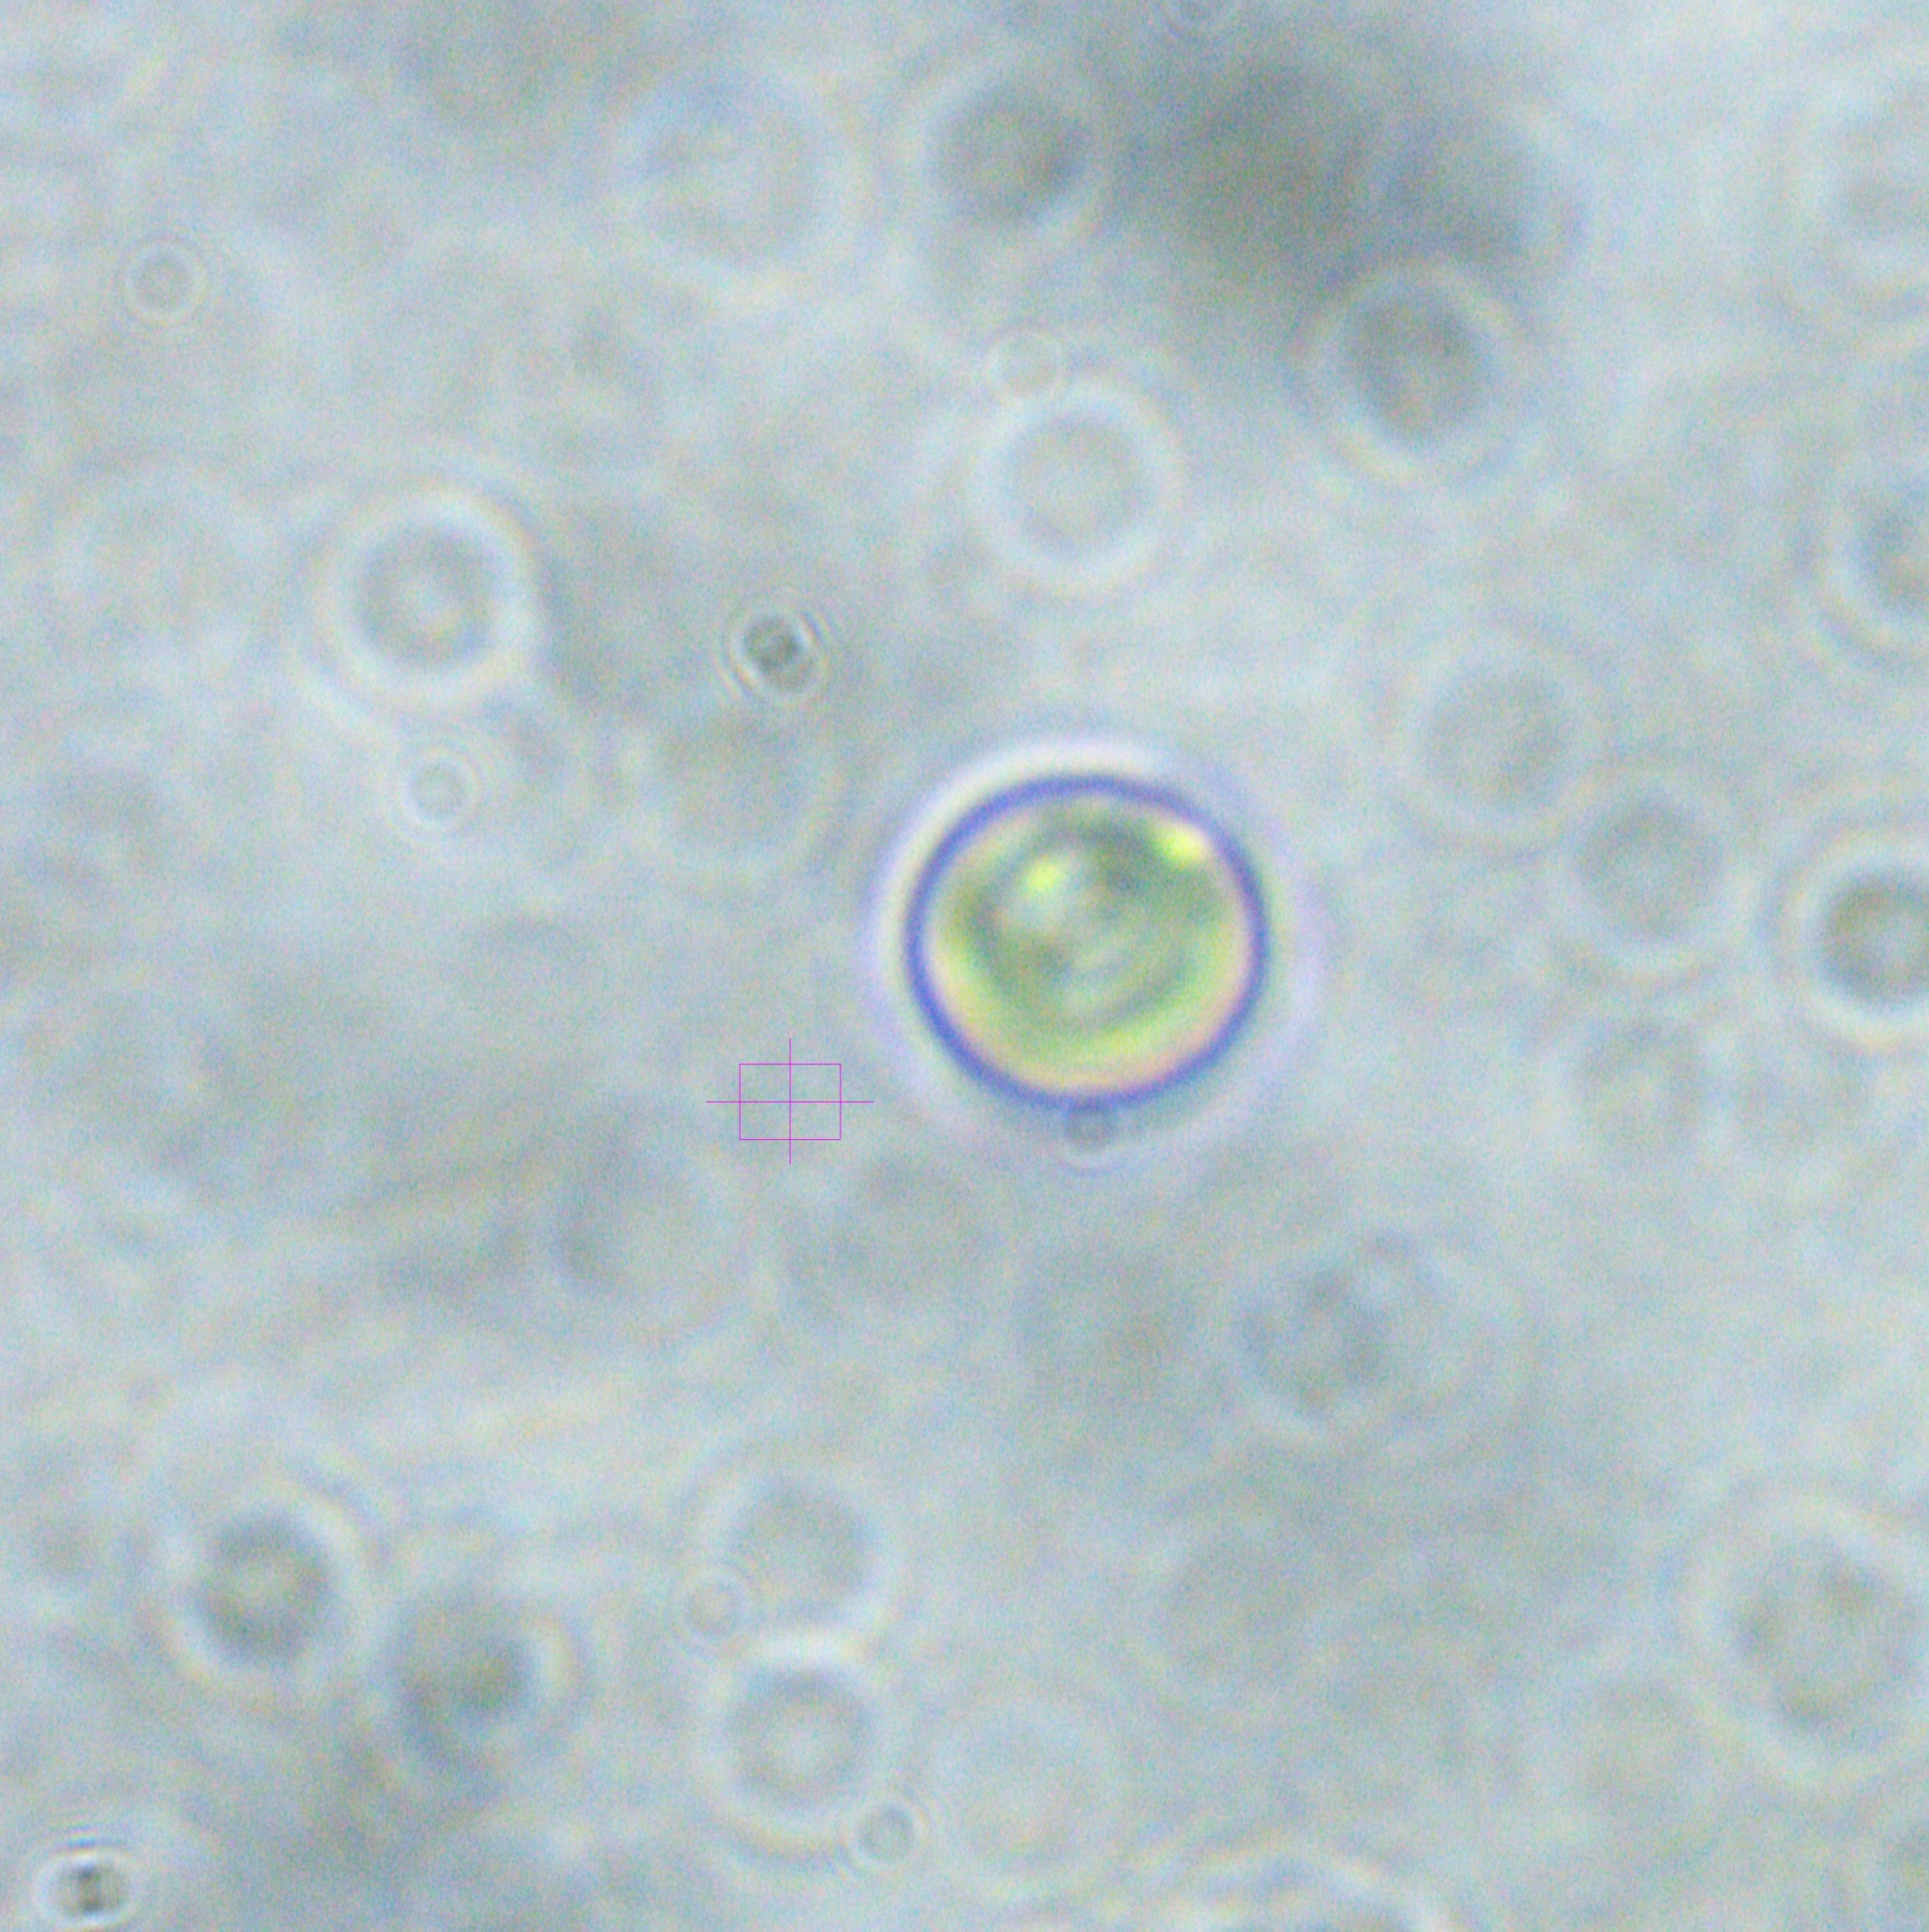
\includegraphics[width=\linewidth]{vaterite_sample.jpg}
		\subcaption{}
	\end{subfigure}
	\begin{subfigure}{0.55\linewidth}
		\includegraphics[width=\linewidth]{rotating_psd.png}
		\subcaption{}
	\end{subfigure}
	\caption{(a)Sample Vaterite sphere suspended in water and trapped by circular polarised trap. (b) Collected power spectrum from rotating Vaterite, peaks in the power spectrum appear at integer multiples of the rotational frequency ($f_{rot} \approx 49.8$ Hz)}
	\label{fig:vaterite}
\end{figure}

As shown by Fig.~\ref{fig:vaterite}(b) the power spectra produced still 
demonstrates a Lorentzian curve but modified with these periodic peaks, 
while the Lorentzian can be loosely fitted to the end tail there exists 
no current model for describing the power spectra. The closest approximation
to this was conducted by \cite{Yogesha2012} where they describe the 
rotational motion of ellipsoidal polystyrene particles. The critical 
assumption being that the particle perfectly rotates in the $x-y$ plane. 
It has long been suspected that birefringent microspheres experience torques 
outside of the $x-y$ plane \cite{Volpe2023} making it very difficult to 
characterise the behaviour of rotating birefringent microspheres without a 
proper understanding of the full optical torque being applied to it.

\subsection{Liquid Crystal Rotors}
Liquid crystals are an intriguing example of materials with mixed phase
properties. Unlike typical solutes such as Glycine, a liquid crystal
can still maintain some degree of order between its individual molecules
while in the liquid state. This is due to the fact that liquid crystals
are constructed of ordered molecules that demonstrate a long range
ordering. There are three main types of liquid crystal transition methods:
Thermotropic crystals will transition to their liquid crystal phase when 
sufficiently heated. Lyotropic materials can undergo this transition due 
to changes in temperature and concentration. And lastly, Metallotropic 
materials - which are composed of both organic and inorganic molecules - 
change phase according to the ratio of organic to inorganic molecules present.
Liquid crystal rotors are rather simple in their production, 4-Heptyl-4-biphenylcarbonitrile (7CB) was purchased from Sigma Aldrich
and a small amount was added to a vial of distilled water. The solution 
was then heated in a water bath to $25^\circ$ in order to transition the
solid crystal into its liquid crystal state. The solution can then be 
loaded onto a sample cover slip and the individual droplets visualised.
The molecules of 7CB will align with a strong electric field, and due to
the spherical droplet geometry the droplets are inherently birefringent. 
\begin{figure}[h!]
	\centering
	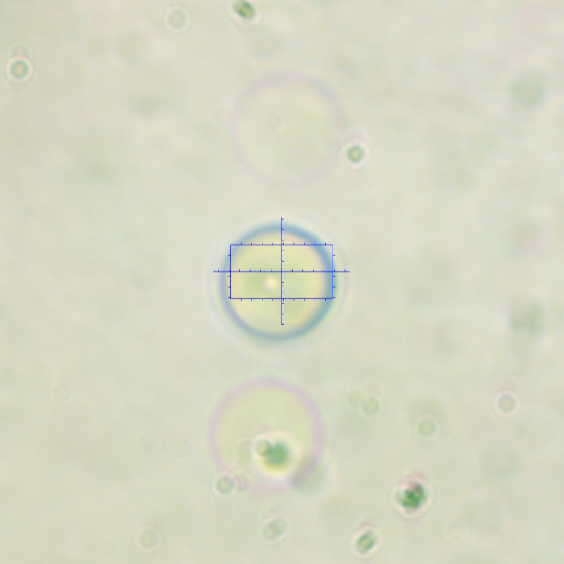
\includegraphics[width=0.5\linewidth]{LC_sample.png}
	\caption{Liquid crystal undergoing rotation due to the circularly polarised trap.} 
\end{figure}

The liquid crystal droplets had a much faster rotation rate than comparable 
Vaterite spheres, due to their higher degree of birefringence and the fact
that the droplets are far closer to perfect spheres making angular momentum
transfer more efficient. 

%%%%%%%%%%%%%%%%%%%%%%%%%%%%%%%%%%%%%%%%%%%%%%%%%%%%%%%%%%%%%%%%%%%%%%%%%%%%%%%%
\section{Rotation of birefringent micro spheres} 
Optical tweezing has often been used for micro-rheology, by computing the
exact forces being exerted on the trapped sphere, one can determine the
local temperature/viscosity of the medium \cite{Millen2014, RodriguezSevilla2018}.
Using a birefringent particle and rotating it within the fluid, the maximum 
rotation rate is due to the fluid drag resisting the torque of the trapping 
beam \cite{RodriguezSevilla2018}. If you want to measure fluid flow you can 
instead use a micro-rotor to see how fluid flow propagates in the medium \cite{Knoener2005}. Likewise, one can use a beam steering arrangement to 
probe the drag force of the fluid, by understanding the trap strength 
(calibrating using a low frequency signal) one can measure the drag force 
experienced by the local fluid \cite{RobertsonAnderson2018}. I

Understanding the fluid velocity around our trapped object is determined 
mostly by the Reynold's number of the system, for a sphere submersed in a 
moving fluid of velocity $U$ this is given by:
\begin{align}
	Re = \frac{\rho UD}{\mu}
\end{align}

Where $D$ is the sphere's diameter, and $\rho$ and $\mu$ are the fluid's 
density and viscosity respectively. In our case we do not have a fluid
moving around a sphere but a sphere moving through the fluid at some 
velocity $U$, assuming a no-slip boundary condition we can model the 
fluid velocity profile based on the velocity of the particle. There are 
two possible avenues for generating shear flow with a trapped particle; 
rotation of birefringent particles, and fluid flow induced by particle motion. 

Rotating birefringent particles are by far the most common method for 
generating and measuring fluid flow in a solution. To see if we can 
even achieve the theoretical maximum shear rate, Vaterite spheres 
were synthesised (see Sec.\ref{sec:vaterite}) submerged in water and 
trapped with the 1064 nm laser at set to 450 mW. The rotation frequency 
was determined using the QPD, and the particle sizes were computed 
by image analysis. With the particle size and rotation frequency, the 
tangential rotation speed is calculated via:
\begin{align}
	\label{eq:birefringent_speed}
	u(r) = \frac{\pi}{4}\frac{d^3}{r^2}\omega
\end{align}

Where $d$ is the particle diameter, $\omega$ is the rotation frequency
reported by the QPD, and $r$ is the distance from the particle's centre. 
Using Eq.\ref{eq:birefringent_speed} we calculated the fluid flow radiating
outward from the centre of the sphere. The shear rate can then be computed
as the partial derivative fluid flow (assuming shearing is generated purely
by the flow field):
\begin{align}
	\label{eq:birefringent_shear}
	\dot{\gamma}(r)=\left|\frac{\delta u(r)}{\delta r} \right|= \frac{\pi}{2}\frac{d^3}{r^3}\omega
\end{align}
%%%%%%%%%%%%%%%%%%%%%%%%%%%%%%%%%%%%%%%%%%%%%%%%%%%%%%%%%%%%%%%%%%%%%%%%%%%%%%%%
%%%%%%%%%%%%%%%%%%%%%%%%%%%%%%%%%%%%%%%%%%%%%%%%%%%%%%%%%%%%%%%%%%%%%%%%%%%%%%%%
\subsection{Estimation of fluid flow around micro-rotors in bulk fluid}
First we determined the upper rotation rate that could be achieved 
using both Vaterite and liquid crystal spheres. Vaterite samples were 
synthesised according to \cite{Parkin2009, Bishop2004} (see sec.~
\ref{sec:vaterite}), and then suspended in distilled water. A sample
of $200\ \mu L$ was pipetted and a single microsphere was captured via
a circular polarised beam. 

Due to Van der Waal's forces some of the microspheres were stuck together, 
fortunately individual sphere's were still present. Multiple microspheres 
were trapped and their rotation rate was determined by looking at the 
peak frequency component of the collected power spectrum. The shear flow
was estimated using eq.\eqref{eq:birefringent_shear} assuming the spheres
were operating in the bulk fluid and away from any boundaries.
\begin{figure}[h!]
	\centering
	\begin{subfigure}{0.75\linewidth}
		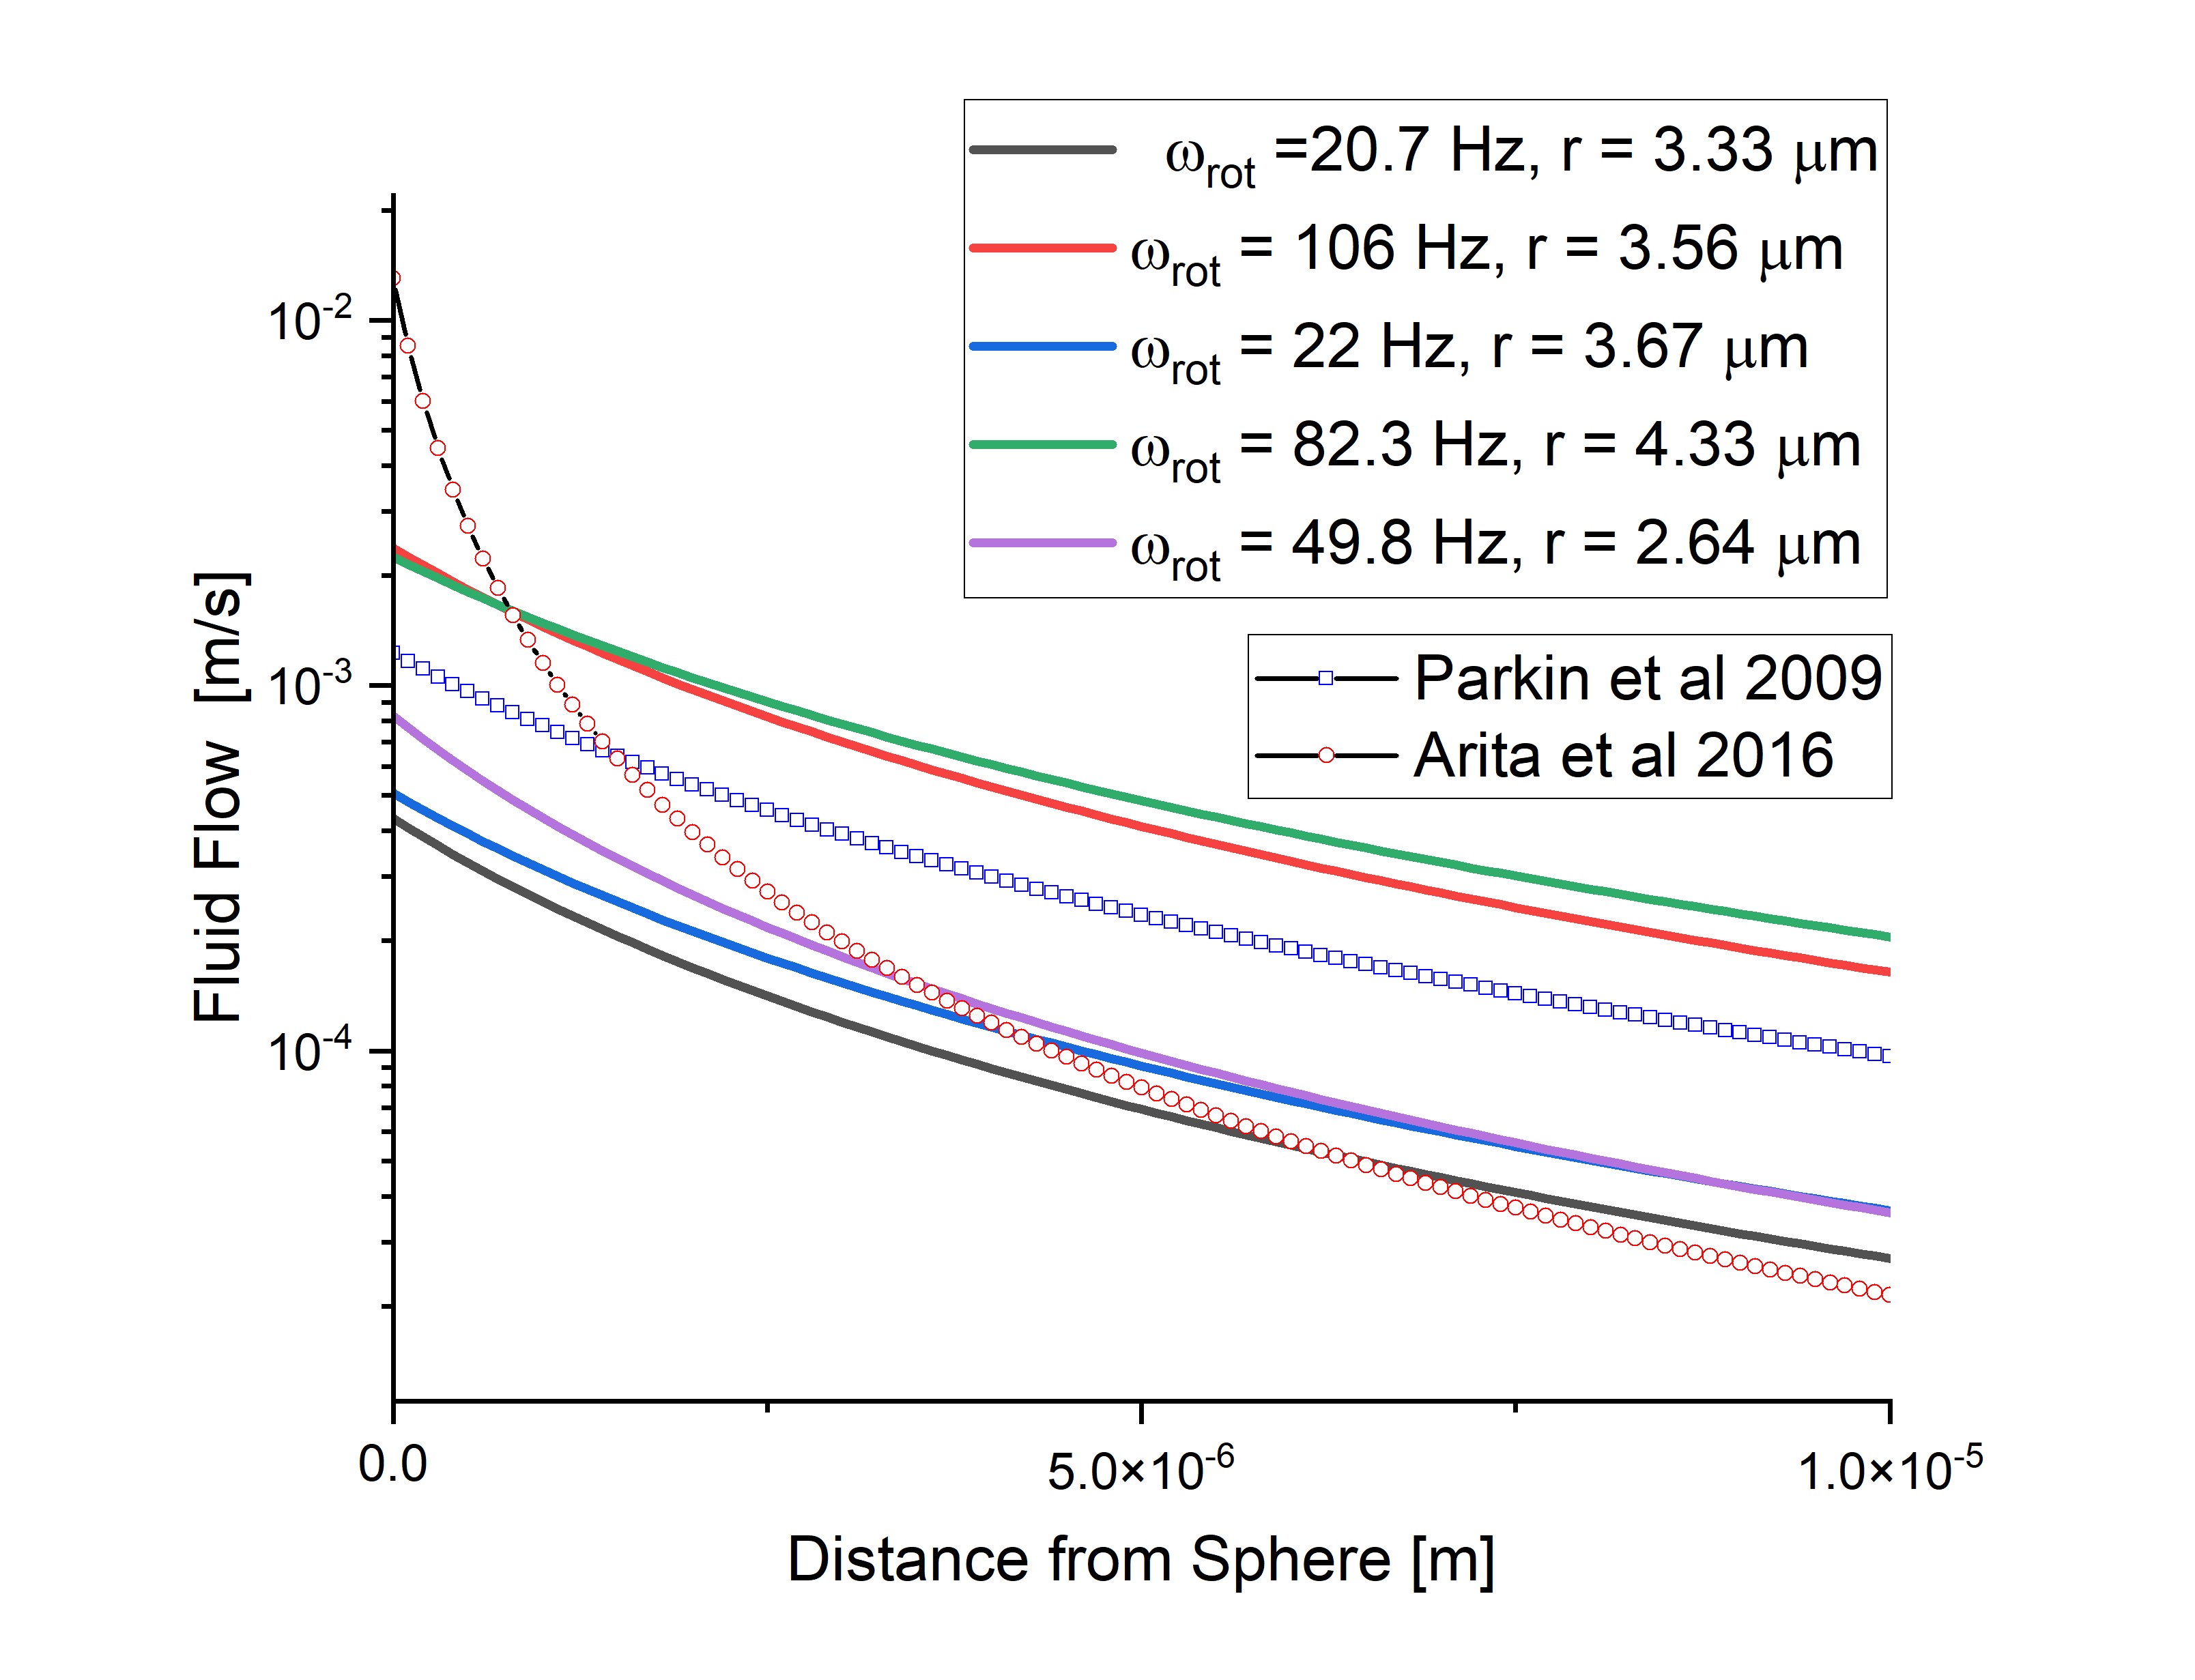
\includegraphics[width=\linewidth]{vaterite_fluid_flow.png}
	\end{subfigure}
	\begin{subfigure}{0.75\linewidth}
		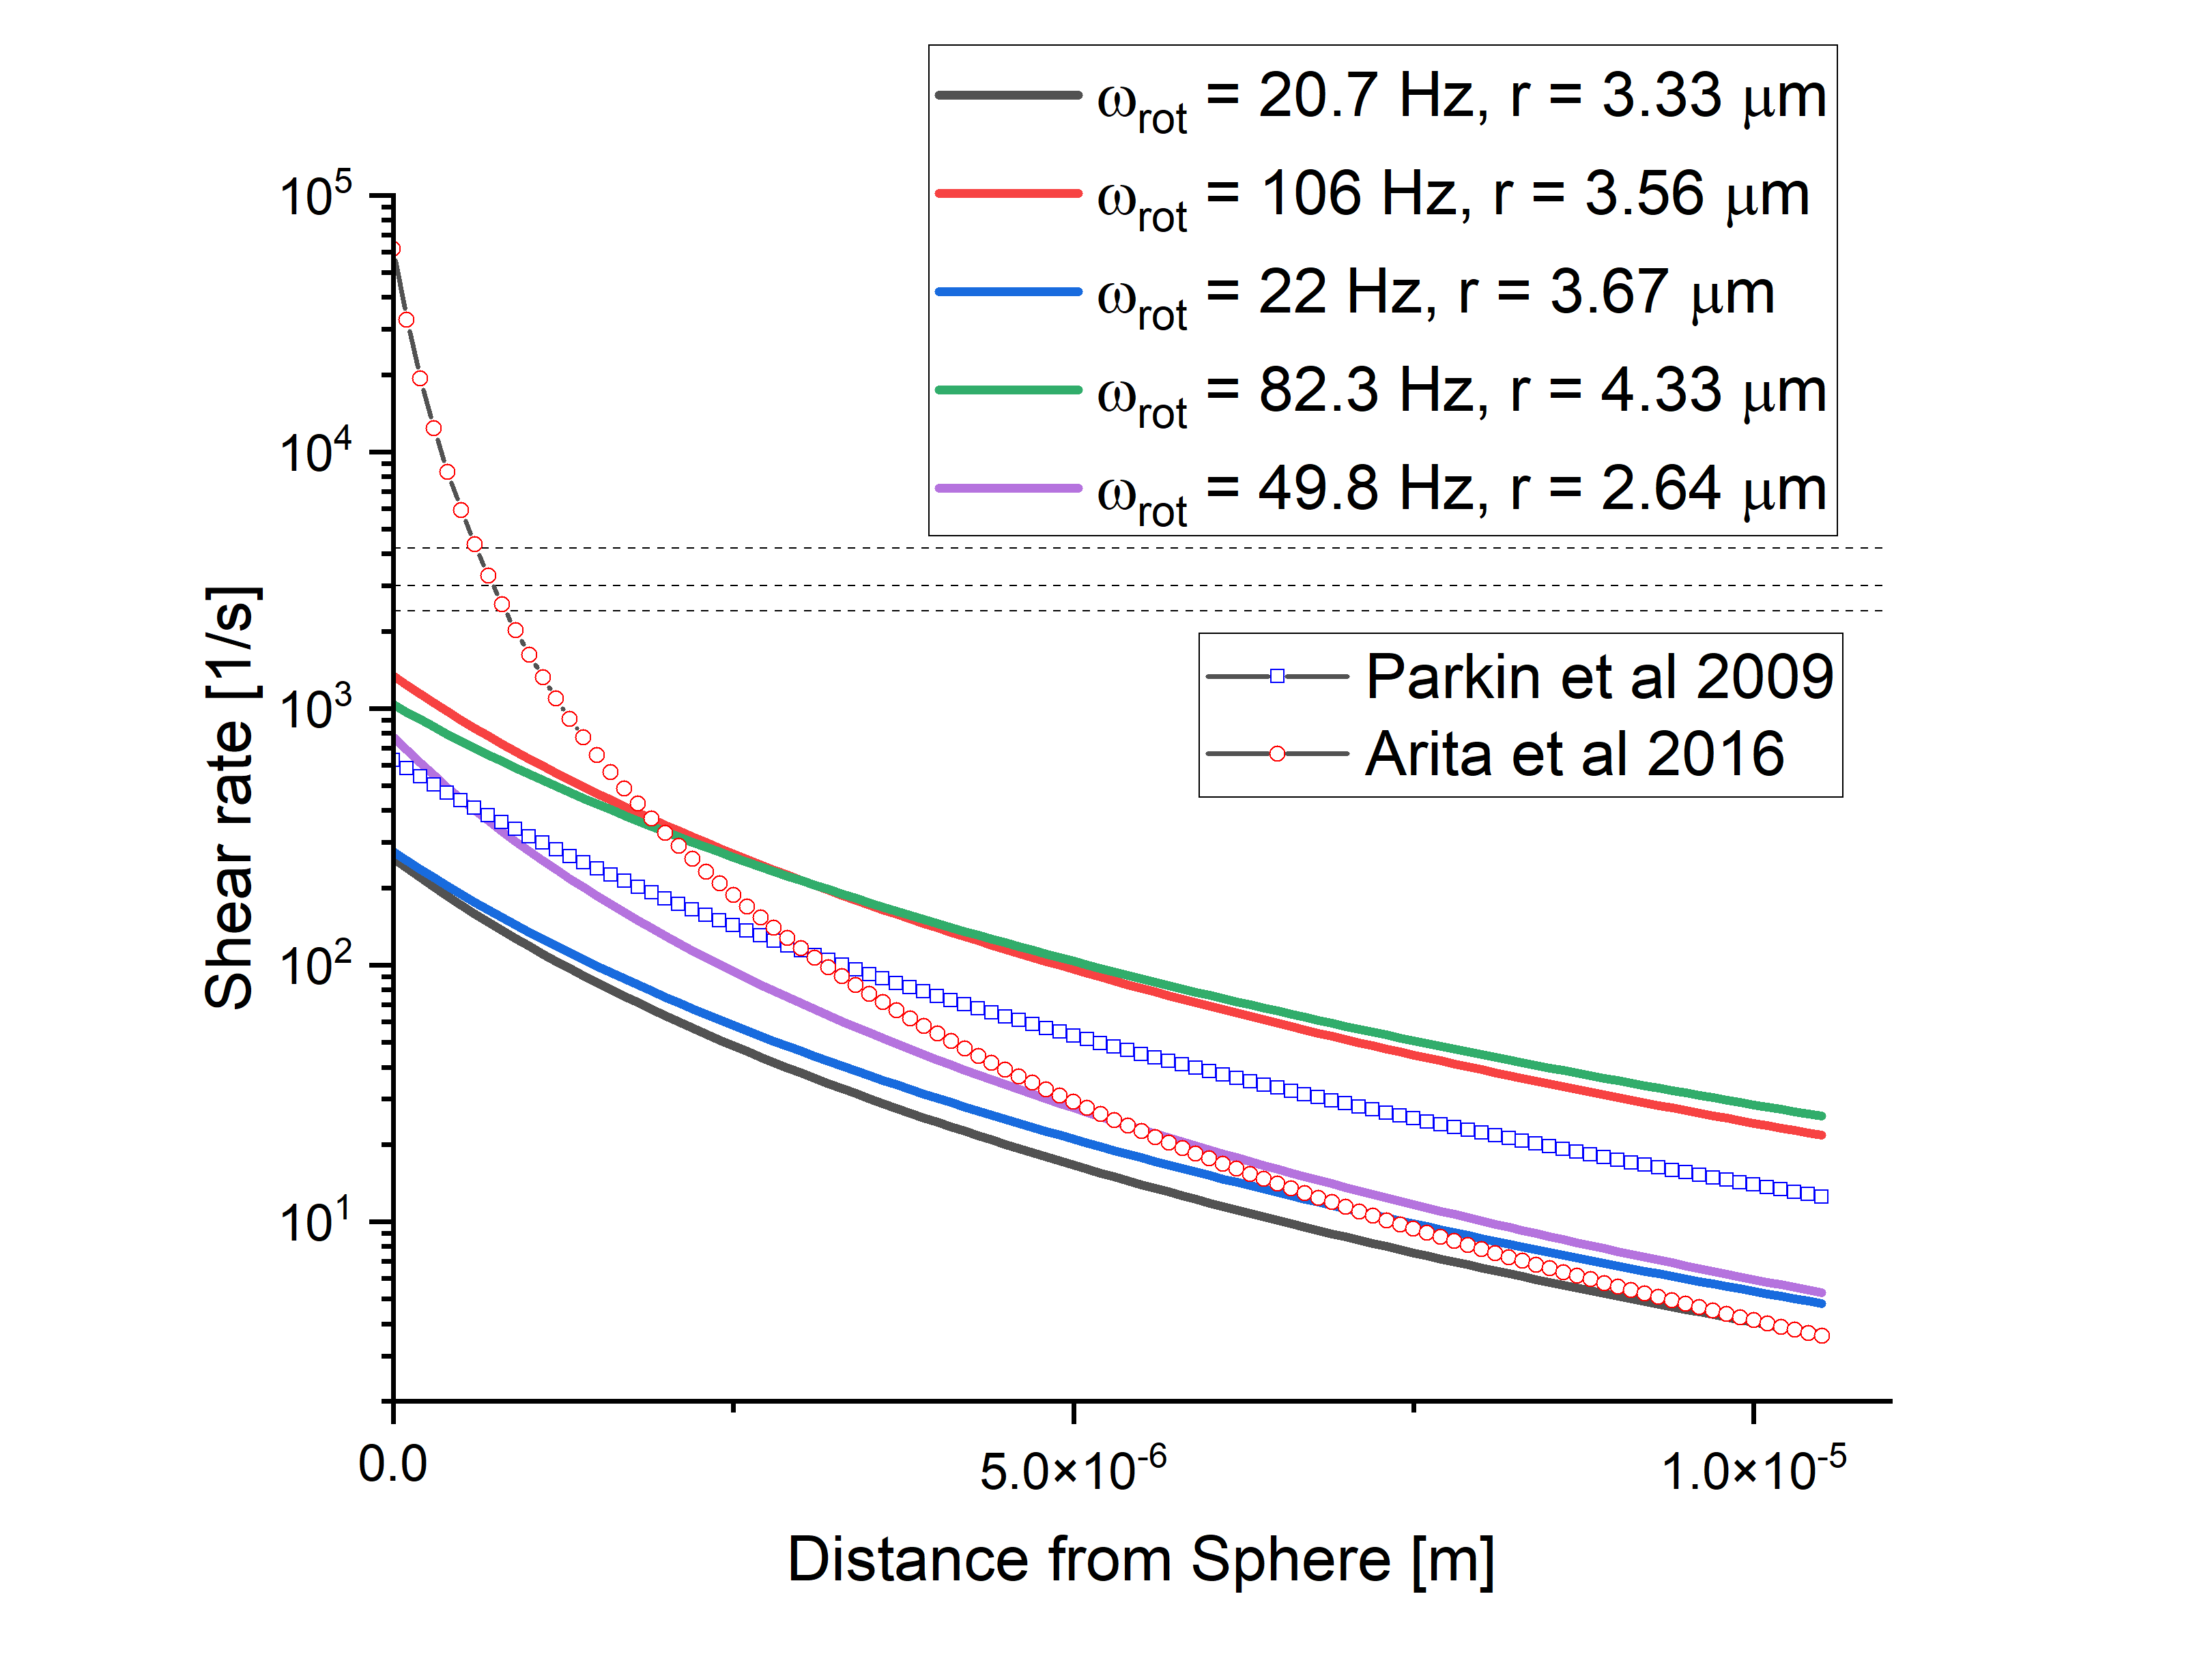
\includegraphics[width=\linewidth]{vaterite_shear_rate.png}
	\end{subfigure}
	\caption{(Top) Fluid flow radiating out from the surface of a rotating 
		Vaterite sphere. (Bottom) Shear rates computed using Eq.\ref{eq:birefringent_shear}, optimal shear rate is of $3000 s^{-1}$ 
		is indicated by the dotted line. Vaterite radii and rotation frequencies 
		are shown, the laser power was kept constant at 450 mW. Reported rotation
		rates, and their corresponding fluid flow and shear rates, for Vaterite 
		are also plotted alongside lab results. Results from \cite{Parkin2009, Arita2016} are included as well.}
	\label{fig:vaterite_shear}
\end{figure}

From Fig.\ref{fig:vaterite_shear} there is not a strong relationship between
particle size and rotation rate, this is contrary to much of the theoretical
predictions that predict an exponential decay with particle size. This can
be in part due to the fact that synthesising perfectly spherical spheres that
have uniform birefringence across the whole population is difficult. Despite 
our best efforts at controlling the growth rate the smallest particle ever 
synthesised was around $3\ \mu m$ in diameter. The Vaterite spheres would 
often stick together while suspended in water after a short period of time. 
The fastest reported rotation rate found during this project was by 
\cite{Arita2016} that achieved a rotation rate of $5\ kHz$, this is plotted 
on Fig~\ref{fig:vaterite_shear} as the dotted line. Even at that extreme a 
rotation rate the region in which nucleation is at its optimal likelihood is 
only $20\ nm$ wide. If instead the micro-rotor was within the vicinity of a
solid boundary, the shear rate would be enhanced due to the no-slip boundary
condition.

\section{Micro-rotors in Supersaturated solution}
If rotation rates in bulk solution are insufficient then a micro-rotor rotating
close to an artificial barrier may be able to improve the shear rate of the 
surrounding fluid. Of course placing a solid barrier in a supersaturated fluid
may well encourage nucleation somewhere on the surface outside of our control.
Instead we chose to use the droplet edge of the supersaturated solution, while
not a hard barrier per say, the molecular mobility close to the droplet edge is
reduced due to surface tension. Furthermore, it has been shown through multiple 
results that nucleation is enhanced at the air-solution interface \cite{Liao2022,
Yuyama2010, Sugiyama2009}. 
\begin{figure}[h!]
	\centering
	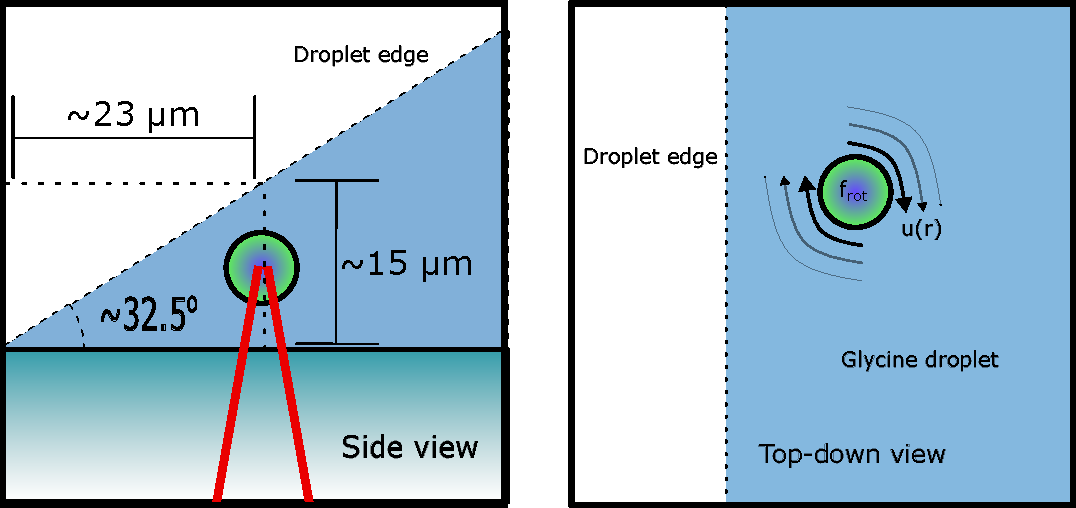
\includegraphics[width=\linewidth]{vaterite_diagram.pdf}
	\caption{Diagram of optical trapping set up for rotating birefringent 
		particles in a supersaturated solution. Left: side view of the 
		trapping set up showing the location of the trap focus at the 
		edge of the droplet of a supersaturated solution. Right: top down 
		view of the glycine droplet with a trapped birefringent particle 
		shown close to edge of the trap. As the particle rotates the drag 
		force from the surrounding fluid generates a flow field around 
		itself (see Eq.~\ref{eq:birefringent_speed}).}
\end{figure}

Supersaturated solutions of glycine and water were prepared and stored in
an incubator prior to use. When ready to be studied $15\ \mu L$ was pipetted 
into the solution and $20\ \mu L$ was pipetted onto the cover slip. A Vaterite
sphere was located, trapped, and moved as close to the droplet edge as possible.
After measuring the microsphere's rotational frequency the sphere was left to
rotate for a period of ten minutes after which, if no nucleation event was 
observed the particle was released. The overall results are catalogued in 
table~\ref{tab:Nucleation}
\begin{table}[h!]
	\centering
	\caption{Results from rotating Vaterite within supersaturated solution of $H_2O$ and Glycine. Solubility concentration for Glycine at $16^\circ$ was $C^*=0.2016g/g$}
	\label{tab:Nucleation}
	\begin{tabular}[width=\textwidth]{|c|c|c|c|}
		\hline
		Super Saturation & Particle radius [$\mu m$] & $\omega$ [Hz] & Nucleation [$\checkmark/\times$]\\
		\hline
		\multirow{3}*{1.01} & 2.34 & 10.4 & $\times$ \\
		\cline{2-4} & 5.67 & 9.63 & $\times$ \\
		\cline{2-4} & 3.26 & 8.46 & $\times$ \\
		\hline
		\multirow{3}*{1.14} & 1.89 & 1.23 & $\times$ \\
		\cline{2-4} & 3.75 & 3.54 & $\times$ \\
		\cline{2-4} & 4.35 & 4.86 & $\times$ \\
		\hline
		\multirow{3}*{1.4} & 3.47 & 0.00 & $\times$ \\
		\cline{2-4} & 1.59 & 0.00 & $\times$ \\
		\cline{2-4} & 6.24 & 0.00 & $\times$ \\
		\hline
		\multirow{3}*{1.45} & 6.32 & 0.00 & $\times$ \\
		\cline{2-4} & 3.68 & 0.00 & $\times$ \\
		\cline{2-4} & 5.43 & 0.00 & $\times$ \\
		\hline
		\multirow{3}*{1.49} & 4.76 & $0.00$ & $\times$ \\
		\cline{2-4} & 7.27 & $0.00$ & $\times$ \\
		\cline{2-4} & 1.52 & $0.00$ & $\times$ \\
		\hline
	\end{tabular}
\end{table}

Trying to trap a particle close to the edge proved more challenging than 
expected. Unlike in previous reports where the beam is focused at the upper
edge of the droplet \cite{Liao2022, Yuyama2010, Sugiyama2022}, we attempted 
trapping into the crook of the droplet. It is suspected that trapping is 
much harder at the interface due to increased surface tension and unpredictable
scattering forces. The closest we could trap a microsphere to the droplet edge 
was in the range of $5-10\mu\ m$, at that distance the fluid flow is so low that 
even the presence of a hard boundary would be insufficient for shearing the 
fluid. Furthermore, as is evident in Table~\ref{tab:Nucleation}, the rotation 
rate drops off significantly with increased supersaturation, due to higher 
fluid viscosities. While in theory a sufficiently focused laser could rotate any microsphere to a fast enough to reach the shear rate predicted by \cite{Debuysschere2023} the localised intensity would be so large that even 
using $D_2O$ would see a significant increase in temperature. 

It is not impossible that fluid shearing could be used in the future to 
localise nucleation; but from these results, using individual micro-rotors 
is not an appropriate method. Firstly, the area of influence is far too small 
to see any noticeable increase in the nucleation rate. And secondly, increased 
fluid viscosity significantly reduces the limits the maximum rotation rate 
possible. If multiple micro-rotors could be trapped in close proximity to one 
another they could create a large region of fluid where nucleation is more likely than the bulk fluid. Micro-rotors have been created that allow for precise
control of suspended micro-particles \cite{Butaite2019} and could potentially be
used to generate sufficient shearing. However these could not be used in this 
project as we lacked the necessary hardware to form multiple gradient traps.  

%%%%%%%%%%%%%%%%%%%%%%%%%%%%%%%%%%%%%%%%%%%%%%%%%%%%%%%%%%%%%%%%%%%%%%%%%%%%%%%%
%%%%%%%%%%%%%%%%%%%%%%%%%%%%%%%%%%%%%%%%%%%%%%%%%%%%%%%%%%%%%%%%%%%%%%%%%%%%%%%%
\section{Shearing via Galvano-mirror manipulation}
An alternative approach to generating fluid shear is to use a galvano-mirror
to rapidly move a trapped particle in a bulk fluid. While typically galvano and gimble mirrors are used to trap multiple particles simultaneously, a single micro sphere can be moved quickly through a fluid along a preset path. The only 
limitation on the particle's speed being the ratio of the trap stiffness to
the drag force. Calculating the shear rate around an individual particle is 
difficult to do precisely but for low Reynolds numbers we can get an adequate approximation.

For a simple circular path one can estimate the sphere's speed by the 
radius of its path and the frequency of its orbit $U = R\omega$; however 
for a more complex path, such as an elliptical orbit the curve needs 
to be parametrised. One can describe the position parameter of a circular 
path as such:

\begin{align}
	r(u) = \left[rcos(2\pi u), rsin(2\pi u), 0 \right]
\end{align}

If we say that $u$ describes time from some initial point we can say $u=t\omega$ 
where omega is the frequency of orbit. Substituting this in and then taking 
the partial derivative of position gives:

\begin{align}
	v(t) = \frac{dr(t)}{dt} = \left[-2\pi r\omega \ sin(2\pi t\omega),
	\ 2\pi r\omega \ cos(2\pi t\omega), 0 \right]
\end{align}

In order to compute U we simply take the magnitude of our velocity. 
For low velocities the fluid flow at the sphere's surface can be computed 
based on its velocity.

\begin{align}
	u_r(r)=-|v(t)|^2\left(1-\frac{3R}{2r}+\frac{R^3}{2r^3}\right)
\end{align}

Where $r$ is the radial distance to that point. Again taking the partial 
derivative we can get the shear rate for a particle moving through the fluid:
\begin{align}
	\dot{\gamma}(r) = \left| \frac{\delta u_r(r)}{\delta r}\right| = |v(t)|^2\left(\frac{3R}{r^2} -\frac{2R^3}{r^4} \right)
	\label{eq:galvo_shear}
\end{align}

Moving a silica bead along an circular path can generate significant fluid 
flow around a larger volume compared to comparable micro-rotors. Using \eqref{eq:galvo_shear} we estimated the shear rate that the surrounding fluid 
would experience at varying speeds. The maximum speed of $7000\ \mu m s^{-1}$
equates to moving the silica bead around a circular path with a frequency of 
$100\ Hz$.
\begin{figure}[h!]
	\centering
	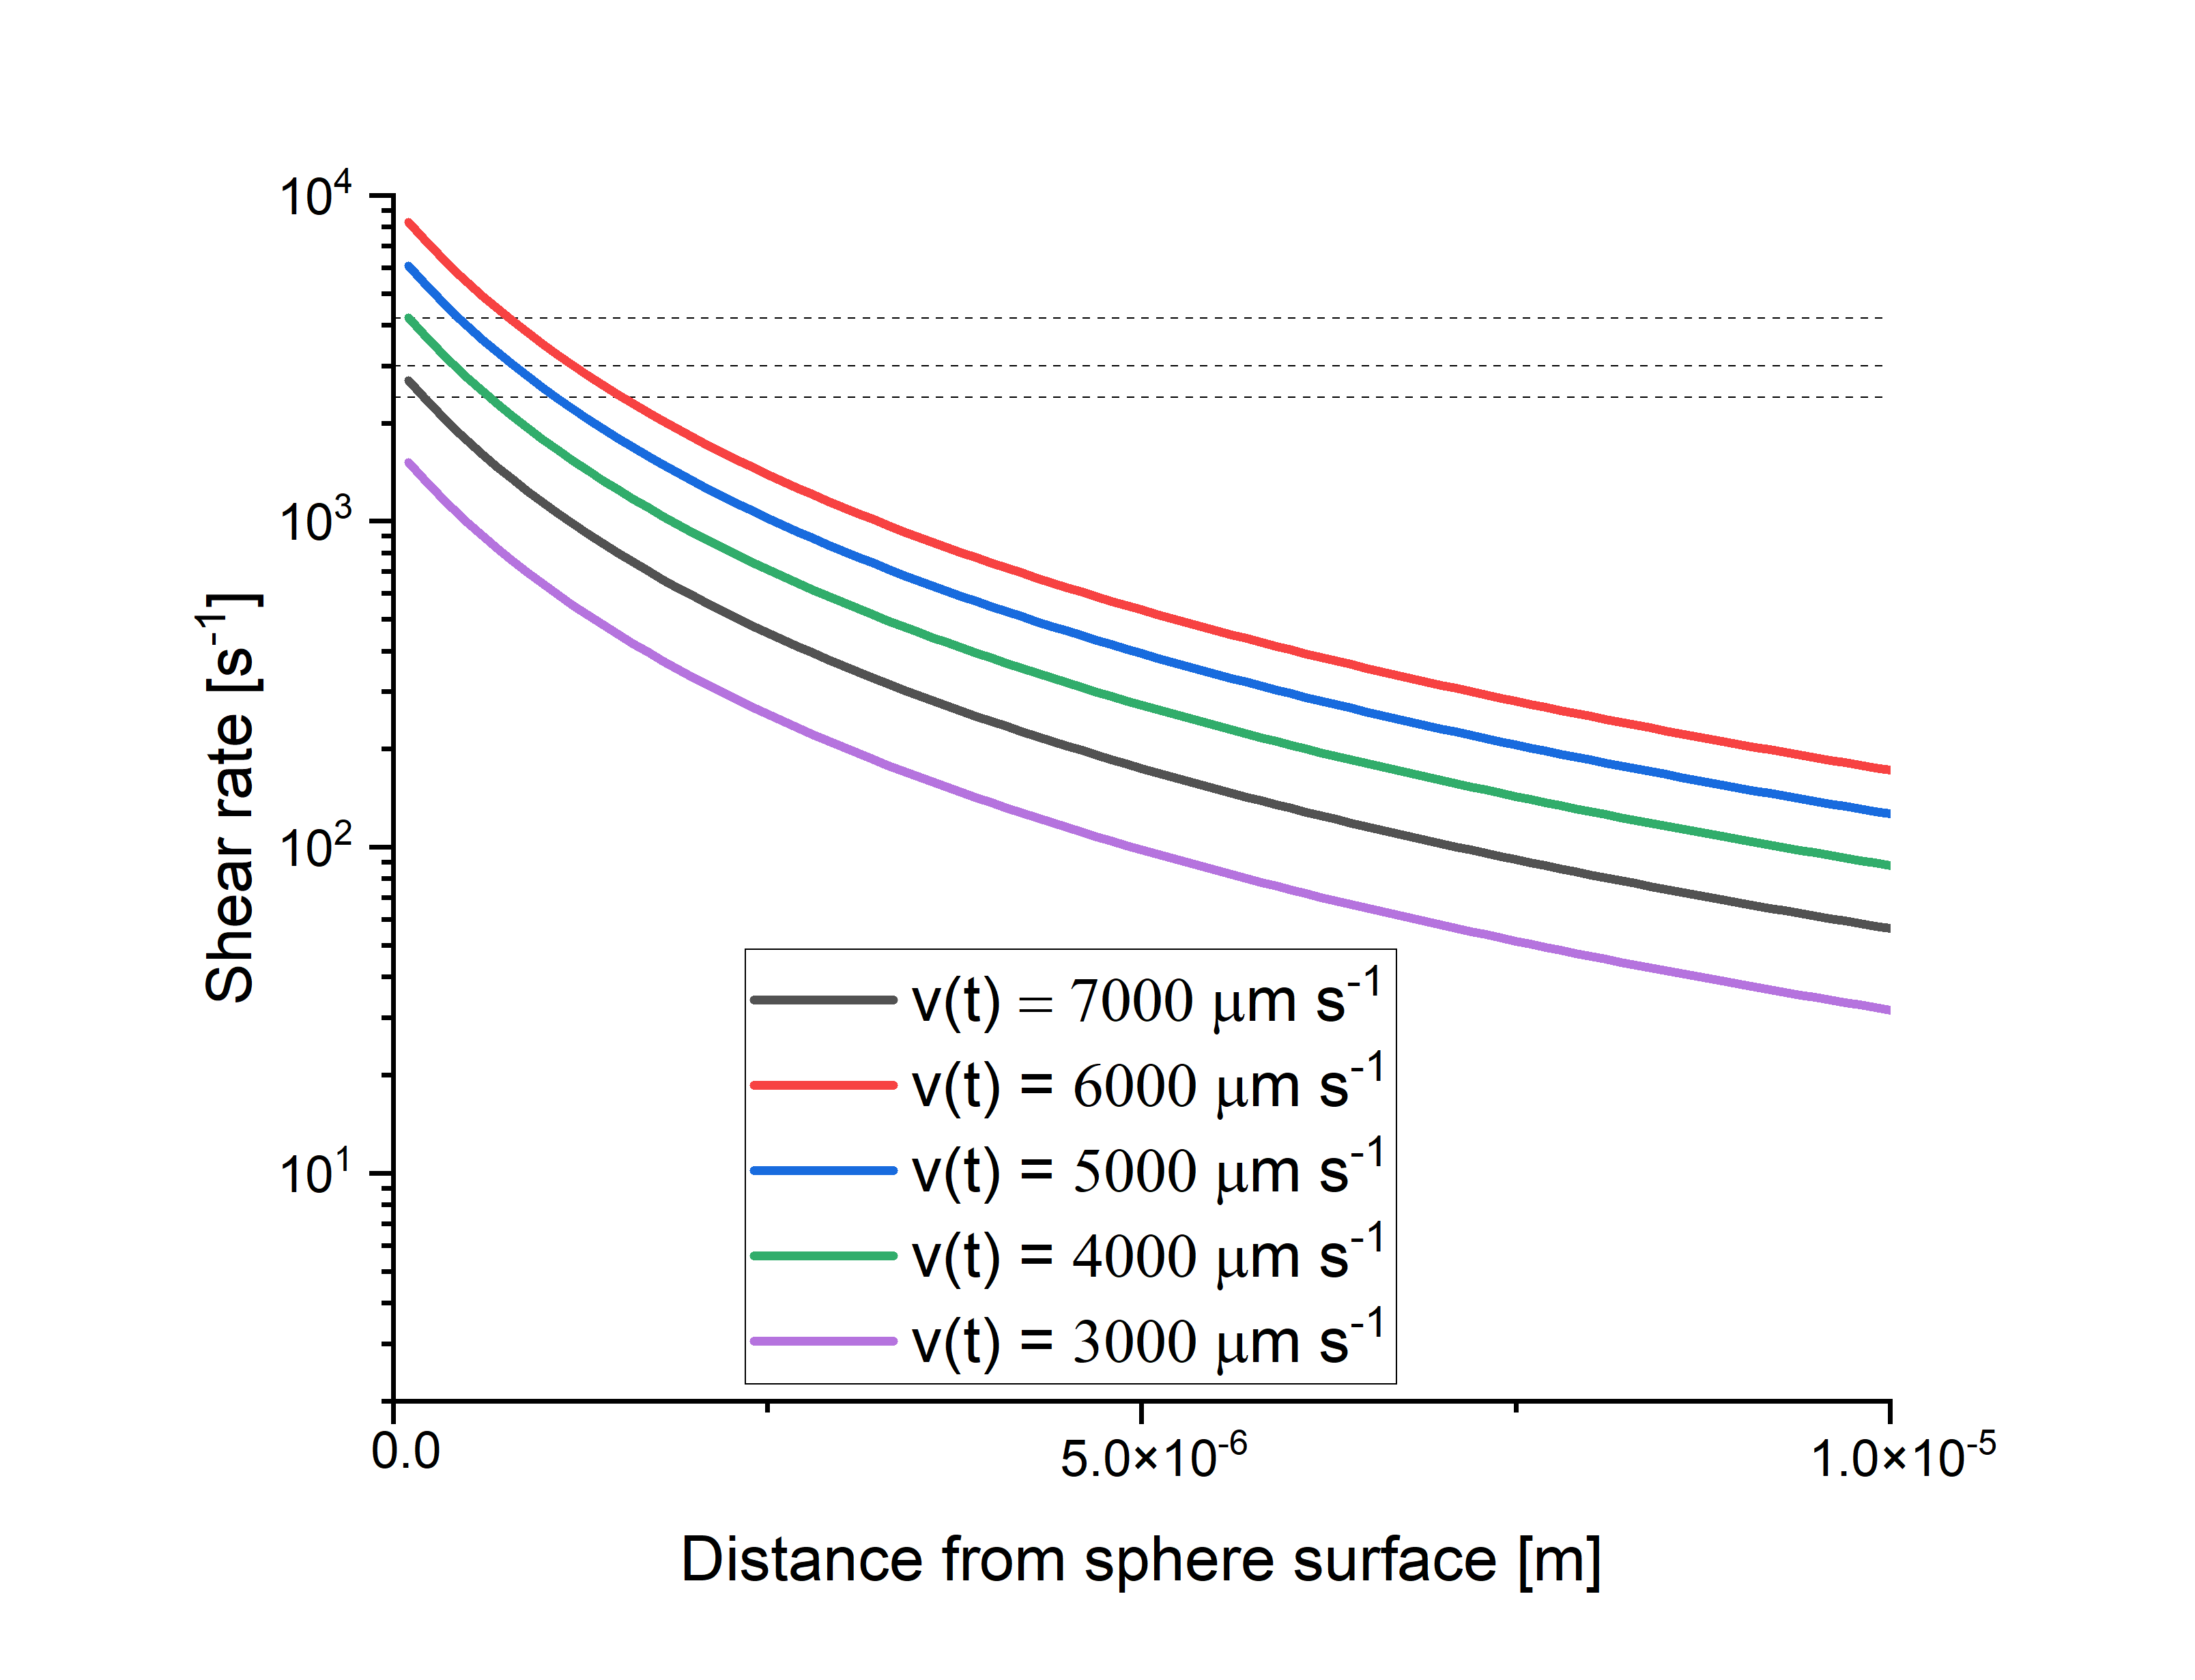
\includegraphics[width=\linewidth]{galvano_shear_rate.png}
	\caption{Shear rate generated by a silica microsphere ($a = 1.57\ \mu m$) 
		in bulk water moving at different speeds. The shear rate is calculated 
		using \eqref{eq:galvo_shear}, with the assumption that the bead is moving
		in a circular path and so the speed is constant through out its path.}
	\label{fig:galvano_shear}
\end{figure}

From figure~\ref{fig:galvano_shear} it is clear that not only is a galvano 
mirror a better option for generating high shear rates but also over a larger 
volume. The only limitation to this method is the effective drag experienced 
by the trapped particle. 

%%%%%%%%%%%%%%%%%%%%%%%%%%%%%%%%%%%%%%%%%%%%%%%%%%%%%%%%%%%%%%%%%%%%%%%%%%%%%
%%%%%%%%%%%%%%%%%%%%%%%%%%%%%%%%%%%%%%%%%%%%%%%%%%%%%%%%%%%%%%%%%%%%%%%%%%%%%
\section{Nucleation with a Stationary and Moving Beam}
As mentioned previously, shearing via optical rotation and particle displacement
did not result in any localised nucleation events even while in the proximity of 
the droplet edge. During the experiments with the galvano-mirror, it was found 
that when no particle was present in the optical trap nucleation events would 
occur while the beam was close to the edge of the droplet, even though the solution
was unsaturated. This has been reported prior \cite{Rungsimanon2010, Liao2022}, 
but was more interesting is how the beam's motion influenced the growth of the 
nucleus.

\subsection{Stationary beam}
\label{sec:stationary}
Consider below in Fig.~\ref{fig:stationary_beam} the frames taken from a nucleation 
event in supersaturated glycine solution ($S=1.03$), the beam is a stationary being 
$\approx3.5 \mu m$ from the droplet edge. After a period of roughly 5 minutes a 
nucleus forms at the trap focus, growing quickly (growth rate was approximated using
imageJ to be on the order of $700\ \mu m^2/min$) from the focal point of the trap 
until after roughly $6$ seconds the crystal escapes. Comparing to previous literature
using optical tweezers shows that the growth rate is only loosely connected to the 
solutions supersaturation. Local conditions play a much larger role in the growth 
rate than just the concentration \cite{Flannigan2023}. A likely reason that the trap 
is escaped is due to the fact that crystal is far too large to be held in place and 
is in fact still growing as the solution is supersaturated. The key take away to 
remember is that the beam has no influence over the crystal shape, instead it 
grows outward from the trap focus. Furthermore, due to the fact that the solution
is supersaturated the crystal growth cannot be contained to the trap focus. Instead 
the crystal escapes as its size exceeds the trap focus. 
\begin{figure}[h!]
	\centering
	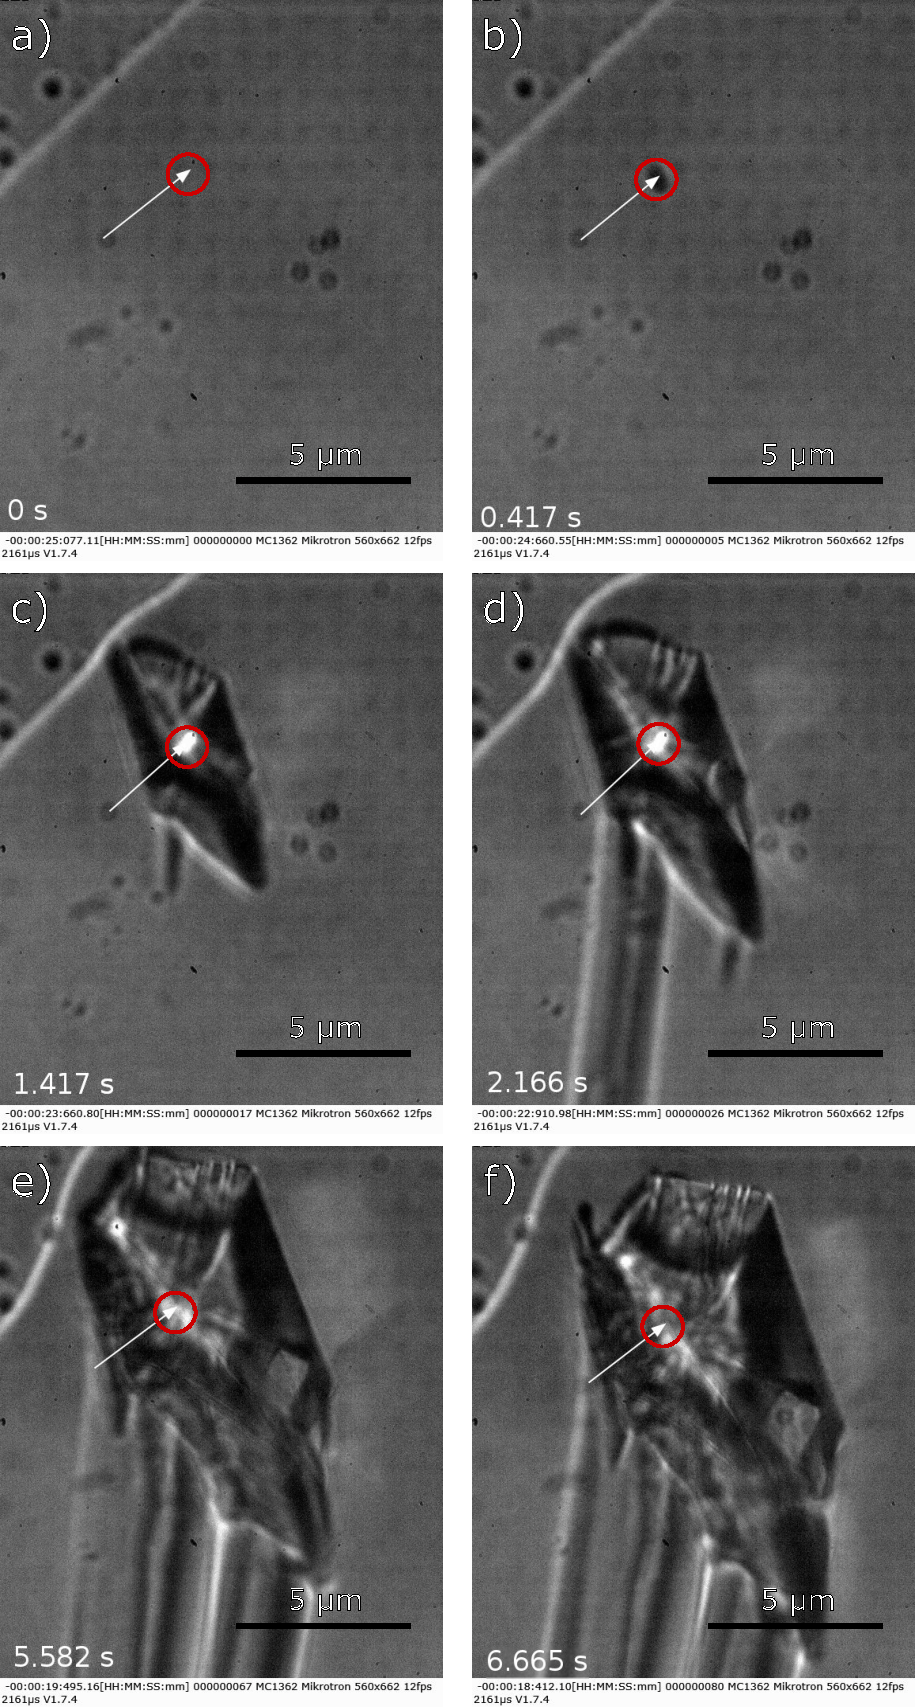
\includegraphics[width=0.63\linewidth]{frames_no_beam_movement.pdf}
	\caption{Laser induced nucleation at the edge of a droplet of supersaturated 
	glycine solution. (b) shows the first instance of a crystal nucleus, growing 
	quickly through (c)-(e) until after $6.665\ s$ the crystal begins to escape 
	the trap.}
	\label{fig:stationary_beam}
\end{figure}

\subsection{Moving Beam}
\label{sec:moving}
To test if a rapidly moving silica bead could generate the necessary shear rate 
for crystal nucleation we wanted to see if a trapped silica bead could be trapped
and moved in an aqueous solution. $20\ \mu L$ of glycine and water ($S=1.03$) was 
added to $10\ \mu L$ of a dilute water-silica mixture making the solution 
unsaturated ($S\approx0.7$). However, due to the beam's motion we instead 
encountered several unexpected results. 

Shown below in Fig.~\ref{fig:eliptical_beam_1} where we have the laser focus 
moving in a small elliptical pattern; interestingly. After a few minutes we 
noted the appearance of several small droplets (see figure~\ref{fig:cluster_trapping}
for a larger example of these droplets). These appear too have a wide distribution
of sizes, unlike silica microspheres which have a uniform radius of $1.57\ 
\mu m$. We surmise these could be small clusters of Glycine that had previously 
been shown to form when the aqueous solutions where irradiated with a 
focused laser \cite{Tsuboi2009, Gowayed2021}. While no droplets are seen 
directly entering the focus a nucleus forms close to the droplet edge, 
unlike in Fig.~\ref{fig:stationary_beam} the crystal does not grow out from 
the focal point evenly. Due to the galvano mirror, the crystal is simultaneously 
being moved by and growing around the focal point of the trap. Because of 
this the crystal nucleus lacks a clear morphology at first. Until roughly 
$20\ s$ the crystal reaches a almost prismatic structure, with further 
irradiation increasing the size.
 
Interestingly the galvano-mirror allows the trap to impart a slight torque 
on the crystal, as shown in fig.~\ref{fig:eliptical_beam_1}(c) and (d), 
where even though the crystal is not directly in the trap focus it rotates 
in the $x-y$ plane and gets trapped again at a corner. The rotation could 
not be due to fluid flow close to the surface of the crystal as the dipole 
moment of individual water molecules is too small to be influenced by an 
optical trap. In figs.\ref{fig:eliptical_beam_1}(e) and (f), the crystal 
growth becomes localised to the corner. The area growth rate between figures \ref{fig:eliptical_beam_1}(a) and (d) was approximated using imageJ at $45.03\ 
\mu m^2 /min$, where as between figures \ref{fig:eliptical_beam_1}(e) and 
(f) the growth rate at that particular edge was estimated at $42.10\ \mu m^2/min$. 
\begin{figure}[h!]
	\centering
	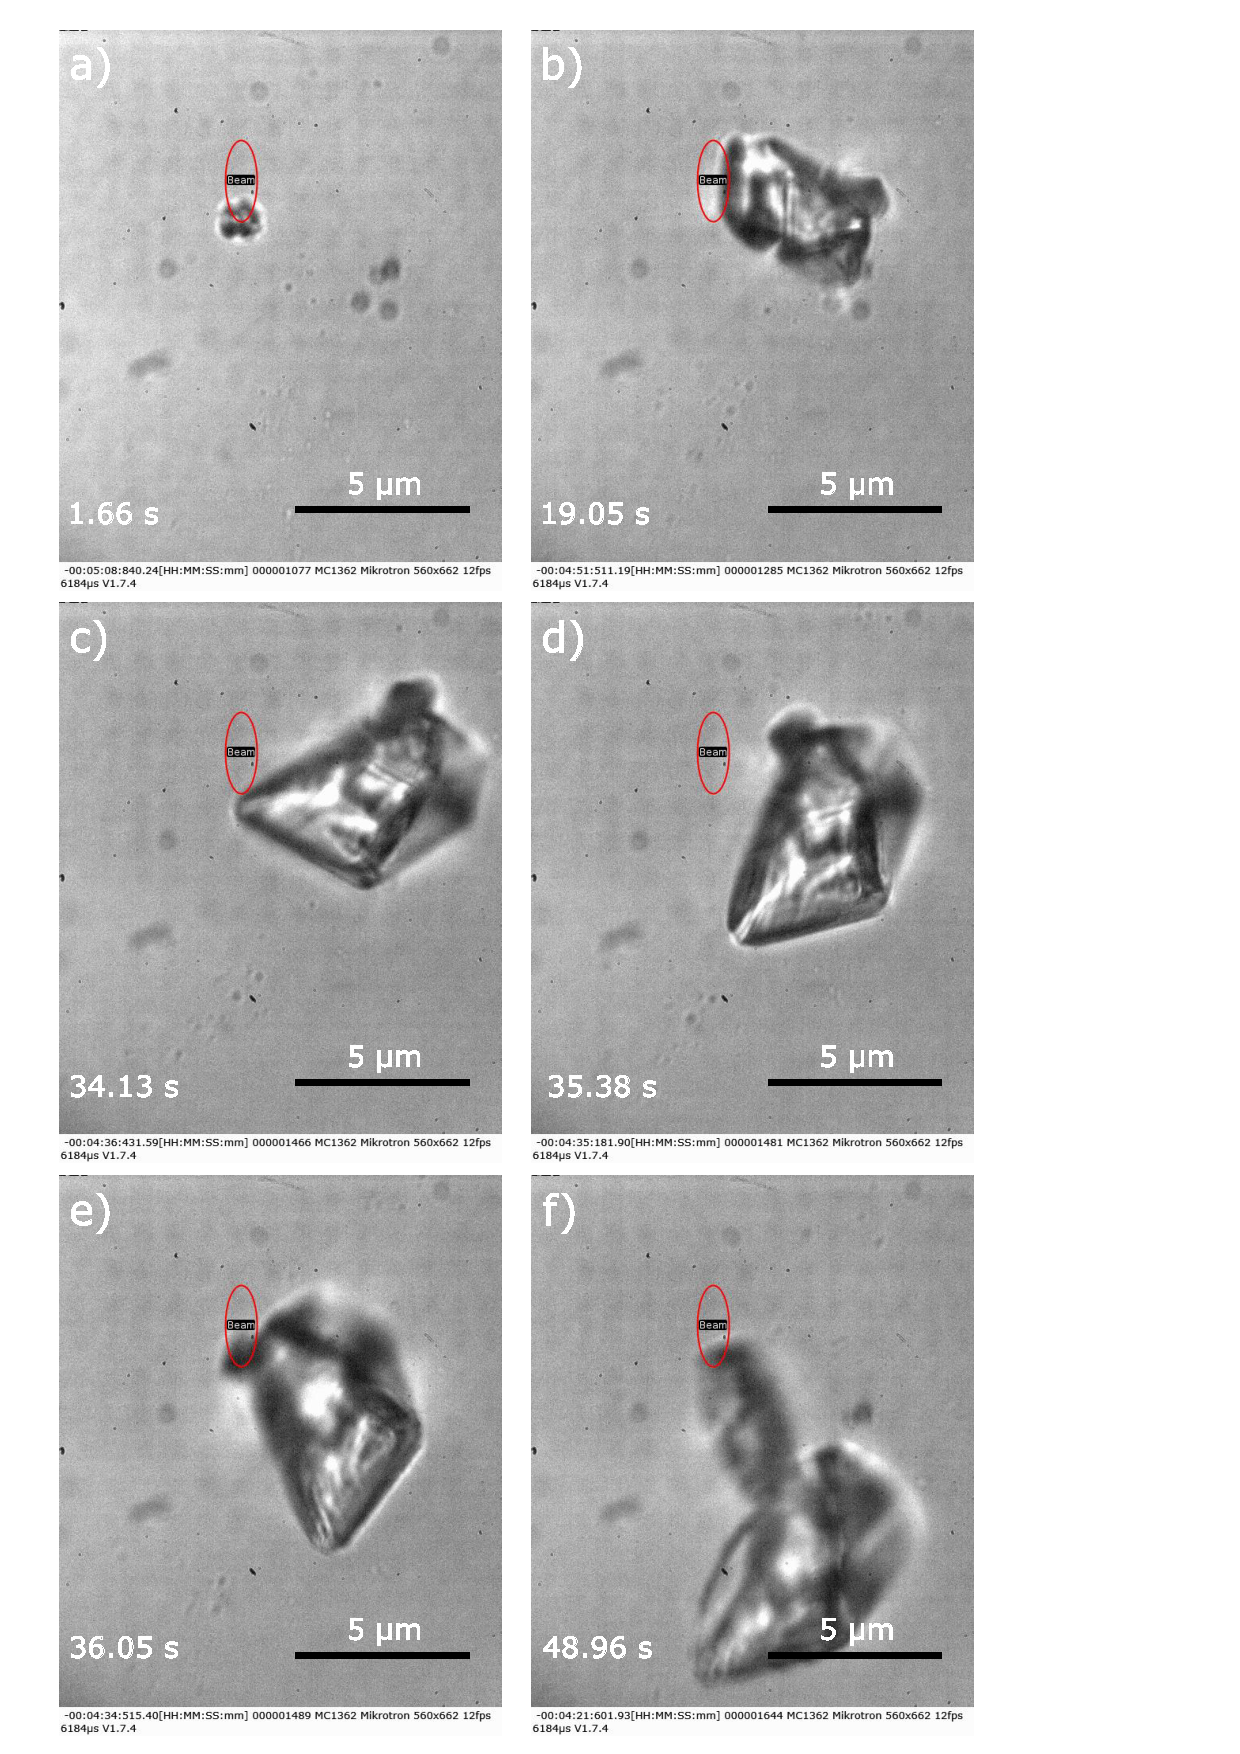
\includegraphics[width=0.85\linewidth]{frames_eliptical_beam.pdf}
	\caption{Frames from a longer video depicting the growth of a nucleus using 
		a moving beam. Initially the crystal shape is amorphous (a) but eventually
		reaches a more regular shape (b). This crystal is still influenced by the
		optical trap as even when not directly irradiated by the laser the crystal
		rotates between (c) and (d). When the laser is focused on a corner the 
		crystal growth is localised to that region, resulting in an elongated 
		section forming between frames (e) and (f).}
	\label{fig:eliptical_beam_1}
\end{figure}
 
Nucleation in undersaturated conditions has been reported previously in $D_2O$ 
\cite{Rungsimanon2010} and $H_2O$ \cite{Flannigan2023}, though not involving a 
moving beam. This modification allows for the crystal growth to be localised to
a specific region of the bulk crystal whereas with a stationary beam there is no
control over the crystal morphology. In fact this allows for a much finer control
over the exact shape of the crystal nucleus, in some cases allowing for growth out
of the viewing plane as shown in 

\begin{figure}
	\centering
\end{figure}


\subsection{Direct trapping of Glycine clusters}
\label{sec:clusters}
One common aspect involving these droplets is the fact when brought to the laser 
focus the droplets would nucleate immediately \cite{Liao2022}. A solution similar 
to Sec~\ref{sec:stationary} was made up, but without any silica droplets. Once 
again the beam was focused close to the droplet edge, this time the galvano mirror
was scanning a circular path (as shown in figure~\ref{fig:cluster_trapping}). 
After a few minutes of irradiation droplets were seen entering the camera frame, 
because no silica had been added these droplets had to be from the glycine solution. Trapping individual droplets did not result in immediate nucleation even after 
several minutes being trapped. Trying to bring two droplets together resulted in nucleation between the two droplets, compared to \ref{sec:stationary} \& 
\ref{sec:moving} the growth is much slower, taking nearly 40 seconds before the 
crystal structure becomes clearer.
\begin{figure}[h!]
	\centering
	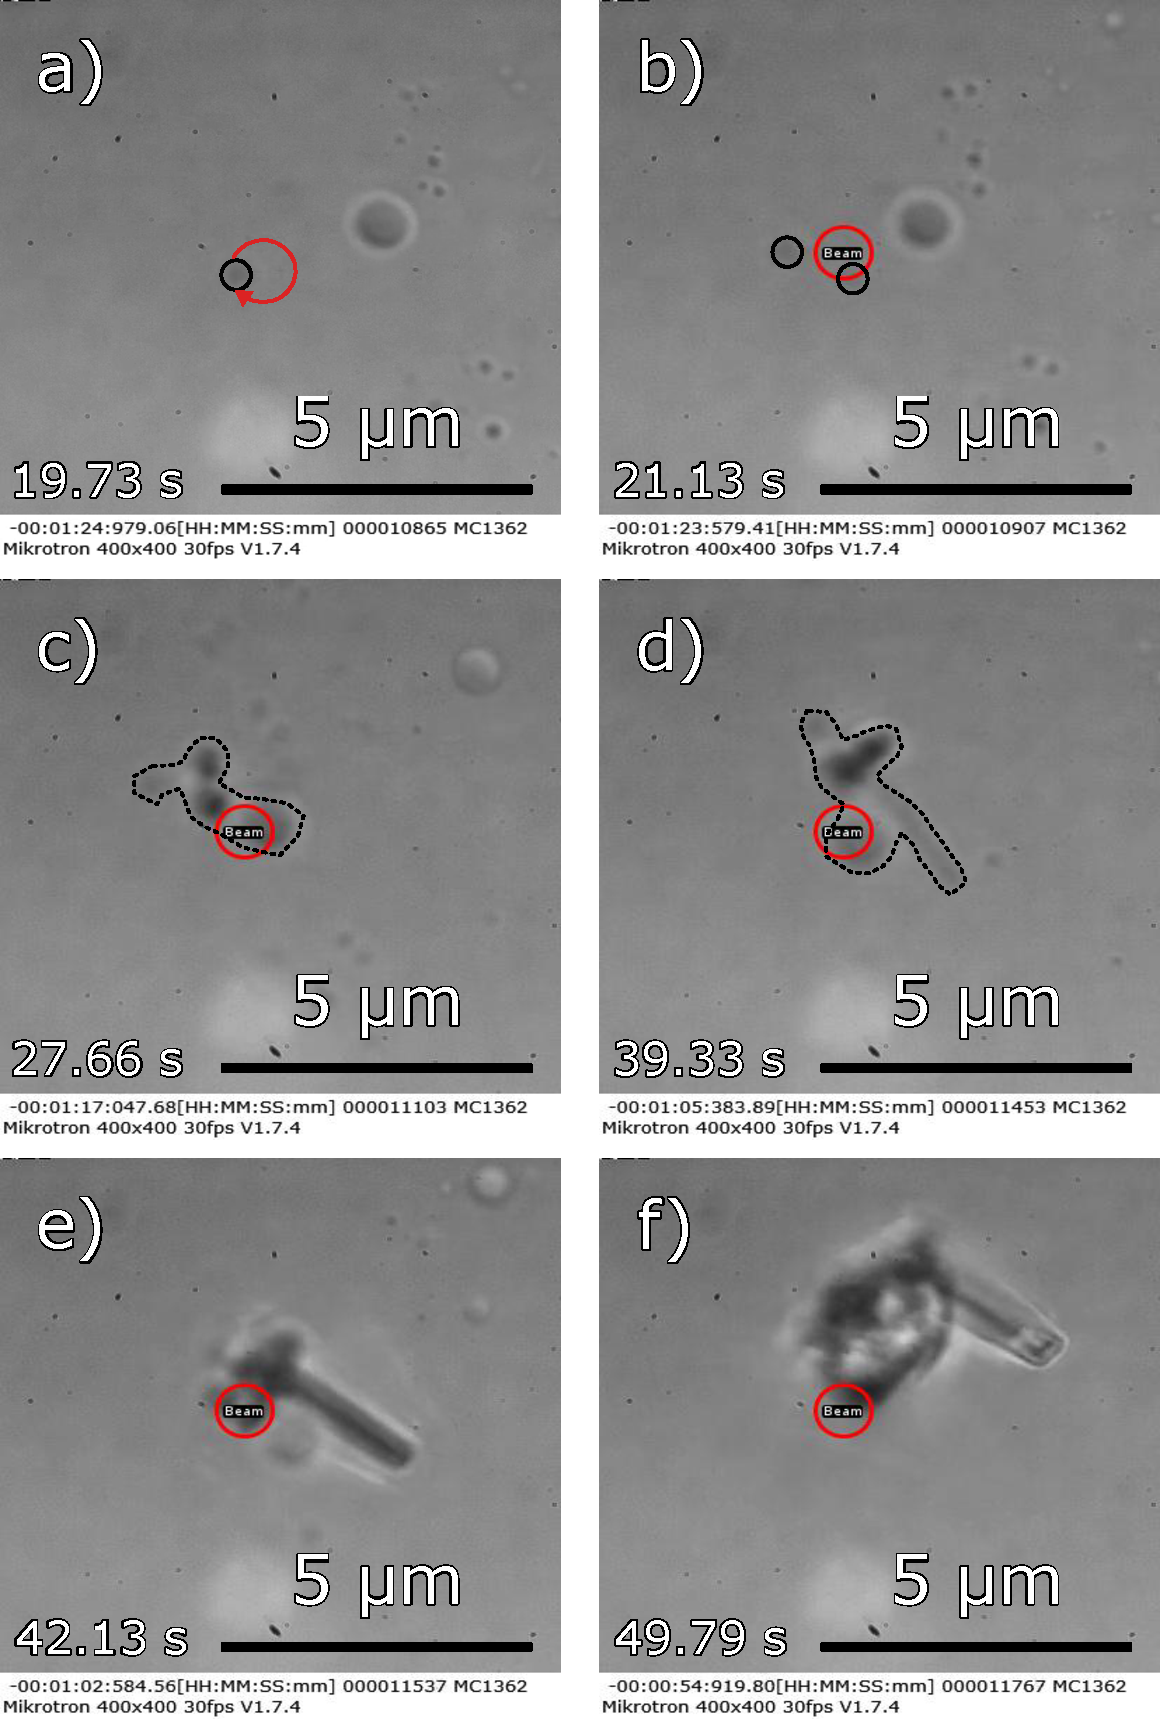
\includegraphics[width=0.7\linewidth]{cluster_trapping.pdf}
	\caption{Frames from a longer video demonstrating the trapping of a glycine 
		droplet. Solution is undersaturated glycine and water (S = 0.86), with the 
		laser power is set at $750\ mW$. (a) shows a trapped droplet (outlined in 
		black) being brought into contact with a larger droplet. (b) upon contact 
		a nucleus can be seen between the two droplets. The growth is rather slow 
		with the crystal having no clear defined morphology through (c) and (d). 
		Between frames (e) and (f) the larger droplet finally joins the main crystal.}
	\label{fig:cluster_trapping}
\end{figure}

The fact that these droplets can be trapped indicates they must have a higher 
refractive index than the surrounding solution. It has been shown that the 
concentration of glycine solution is correlated with the refractive indices 
of the liquid \cite{Gowayed2021, Orttung1963}. This suggests that these droplets 
serve to provide solute material to the bulk crystal. 


\subsection{Influence of a moving beam front on seed crystals}
One potential application of this phenomena would be in using a 
moving the moving beam front as a method for shaping the final
crystal morphology. Glycine seed crystals were grown via 
evaporative crystallisation over night. The resultant crystals
were as wide as $0.5 mm$ in some cases. Individual crystals were 
collected and suspended in a water + glycine solution ($S = 1.001$)
and the laser was switched on.  

\section{Summary of Moving Beam Phenomena}
To summarise, the introduction of a moving beam helps to accelerate the 
local growth of a newly formed crystal. This is due to the presence of 
glycine droplets that accumulate near the interface between the liquid 
solution and air. The theory behind the localised growth can be summarised 
thusly.

Initial nucleation is similar to typical optical trapping induced nucleation,
with the air solution interface limiting the molecular mobility of the solute
molecules \cite{Liao2022, Sugiyama2009, Gowayed2021}. The moving beam front 
can influence the motion of the nucleus initially, but eventually the drag 
force means the crystal is not moved by the optical trap. Localised crystal
growth occurs when the trap is close to or partially over the interface of 
the crystal (see figure~\ref{fig:local_nucleation}(a)). As shown in \ref{sec:clusters}, the optical trap can manipulate these droplets similar 
to microspheres. When in close proximity to the trap these droplets are 
brought towards the crystal surface (see figure~\ref{fig:local_nucleation}(b)). 
These provide material that grows the crystal around that region (see figure~\ref{fig:local_nucleation}(c)). Eventually the local solution is either 
depleted of solute material or the crystal front has grown to fully encompass 
the trap, preventing further growth (see figure~\ref{fig:local_nucleation}(d)). 
\begin{figure}[h!]
	\centering
	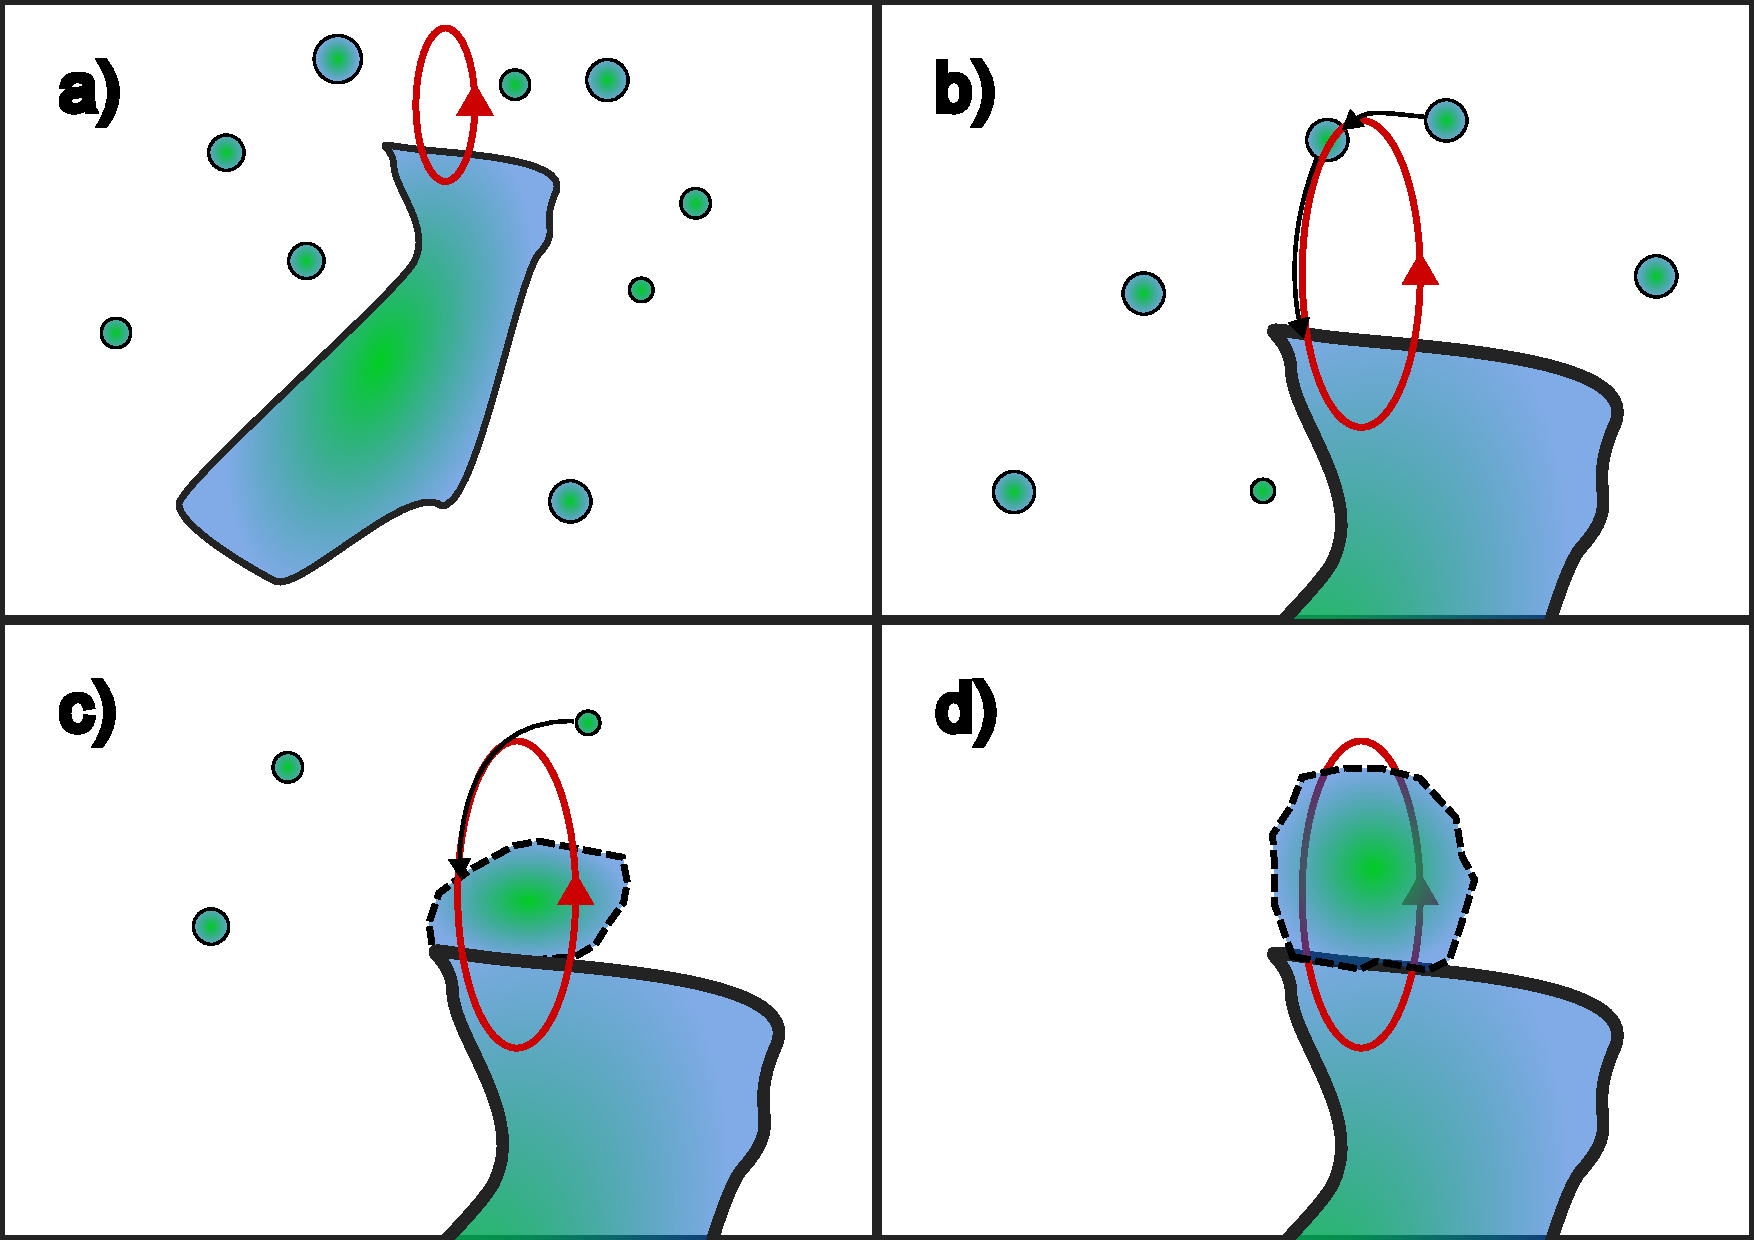
\includegraphics[width=0.8\linewidth]{galvano_diagram.pdf}
	\caption{Diagram outlining how a moving beam assists in the growth of a crystal
		nucleus. (a) a crystal nucleus is partially trapped by a moving beam with 
		solute droplets close to its surface. (b) droplets close to the laser
		focus are drawn in by gradient forces and moved towards the crystal surface.
		(c) these droplets provide material to the main crystal, resulting in
		localised growth around the laser focus. (d) eventually the crystal area 
		either fully surrounds the laser focus or the solution surrounding the laser
		is depleted of solute material.}
	\label{fig:local_nucleation}
\end{figure}

The reason the seed crystals saw no further crystal growth when irradiated 
with the trap is due to the fact that these experiments were carried out 
in a bulk solution, absent of any interfaces. As such the clusters seen in
\ref{sec:moving} \& \ref{sec:clusters} are not present and cannot provide
material to accelerate crystal growth.

There are still several factors that need to be investigated, but due to time
constraints it was not possible to properly study this phenomena. Firstly, 
there is the question of what conditions result in the production of concentrated
droplets, it is not clear if the presence of a laser is required or if these
droplets naturally occurring. Prior literature would suggest that the laser is 
required \cite{Liao2022, Tsuboi2009}, but this would not explain why in many 
cases the droplets are found far outside the influence of the optical trap. It
has been suggested that optical traps can attract microspheres over a wider 
area, but it is hard to say that this would result in the creation of liquid 
droplets \cite{Yi2021}.

Secondly, there is the question of how these droplets supply material to the 
bulk crystal. In some instances it is clear that the droplets are being drawn 
into the trap, however, in other instances while there are no droplets close to
the vicinity of the optical trap the crystal continues to grow. If these droplets
are a necessary precursor to induce crystal nucleation then understanding how
they provide materials to the bulk crystal may help with our understanding of 
the kinetics of multi-step nucleation. 

\section{Conclusion}

